% Journal of Forensic Sciences -- anonymised manuscript file (no author
% information; the title page is a separate file, titlepage.tex).
% Overleaf: Compiler pdfLaTeX (any TeX Live version). No BibTeX run is
% needed: the reference list below is already in JFS (Vancouver/NLM) style.
\documentclass[12pt]{article}
% ---------------------------------------------------------------- packages
\usepackage[T1]{fontenc}
\usepackage[utf8]{inputenc}
\usepackage{mathptmx}                 % Times text and maths
\usepackage[scaled=0.92]{helvet}      % Helvetica (line numbers)
\usepackage{courier}                  % Courier (file names)
\usepackage[letterpaper,margin=1in]{geometry}
\usepackage{amsmath,amssymb}
\usepackage{graphicx}
\usepackage[table]{xcolor}
\usepackage{booktabs,array,makecell}
\usepackage{adjustbox}
\usepackage{pifont}
\usepackage{algorithm}
\usepackage{algpseudocode}
\usepackage{tcolorbox}
\usepackage{float}
\usepackage{etoolbox}
\usepackage{setspace}
\usepackage{caption}
\usepackage{titlesec}
\usepackage[numbers,square,sort&compress]{natbib}
\usepackage{lineno}
\usepackage{xurl}
\urlstyle{same}
\usepackage[hidelinks]{hyperref}
\hypersetup{pdftitle={Structure-aware forgery detection for Aadhaar and Permanent Account Number cards},
  pdfauthor={}, pdfsubject={}, pdfkeywords={}, pdfcreator={}}

% ---------------------------------------------------------------- JFS layout
% Double spacing throughout, including abstract, highlights, references
% and table and figure legends (JFS Information for Authors, June 2025).
\doublespacing
\setlength{\parindent}{1.5em}
\pagestyle{plain}

% Headings: all caps and bold; subheadings upper/lower case, italic, not
% bold; sub-subheadings upper/lower case, plain text.
\setcounter{secnumdepth}{3}
\titleformat{\section}{\normalfont\bfseries}{\thesection}{0.6em}{\MakeUppercase}
\titleformat{\subsection}{\normalfont\itshape}{\thesubsection}{0.6em}{}
\titleformat{\subsubsection}{\normalfont}{\thesubsubsection}{0.6em}{}
\titleformat{\paragraph}[runin]{\normalfont\itshape}{}{0pt}{}
\titlespacing*{\section}{0pt}{1.2\baselineskip}{0.4\baselineskip}
\titlespacing*{\subsection}{0pt}{0.9\baselineskip}{0.3\baselineskip}
\titlespacing*{\subsubsection}{0pt}{0.7\baselineskip}{0.2\baselineskip}
\titlespacing*{\paragraph}{0pt}{0.4\baselineskip}{0.5em}

% Legends: "TABLE 1 Legend text." and "FIGURE 1 Legend text."
\captionsetup{font=doublespacing, labelfont=bf, labelsep=space,
  justification=justified, singlelinecheck=false, skip=6pt}
\captionsetup[table]{name=TABLE, position=top}
\captionsetup[figure]{name=FIGURE}

% Tables: single-spaced body, 10 pt; each tabular is shrunk only if it is
% wider than the text (adjustbox, max width).
\AtBeginEnvironment{table}{\let\scriptsize\footnotesize\let\tiny\scriptsize}

% References: bold "References" heading, numbered "1.", "2.", ...
\renewcommand{\bibsection}{\par\bigskip\noindent\textbf{References}\par}
\renewcommand{\bibnumfmt}[1]{#1.}
\setlength{\bibsep}{0pt}

% ---------------------------------------------------------------- paper macros
\algtext*{EndFor}% omit "end for" / "end if" lines in the algorithms
\algtext*{EndIf}

\definecolor{cvis}{HTML}{2F6DB5}    % visual branch
\definecolor{crule}{HTML}{D27A1E}   % structural / semantic branch
\definecolor{cfuse}{HTML}{2E8B57}   % fusion
\definecolor{cbad}{HTML}{C0392B}    % failure / forgery
\definecolor{cink}{HTML}{2B2B2B}
\definecolor{cgrey}{HTML}{6B7280}

\newcommand{\cmark}{\textcolor{cfuse}{\ding{51}}}
\newcommand{\xmark}{\textcolor{cbad}{\ding{55}}}

% Research-question box (Section 1)
\newtcolorbox{rqbox}[1]{colback=white, colframe=black!60,
  boxrule=0.5pt, arc=0pt, left=8pt, right=8pt, top=5pt, bottom=5pt,
  fonttitle=\bfseries\normalsize, coltitle=black, colbacktitle=black!8,
  title=#1, fontupper=\normalsize}

% Auto-generated by scripts/export_latex.py -- do not edit by hand.
\newcommand{\dsPersons}{300}
\newcommand{\dsDocuments}{3{,}600}
\newcommand{\dsImages}{10{,}800}
\newcommand{\dsGenuine}{3{,}600}
\newcommand{\dsForged}{7{,}200}
\newcommand{\dsGiB}{0.88}
\newcommand{\dsNq}{3}
\newcommand{\dsTrainImg}{7{,}560}
\newcommand{\dsValImg}{1{,}620}
\newcommand{\dsTestImg}{1{,}620}
\newcommand{\dsTrainPer}{210}
\newcommand{\dsValPer}{45}
\newcommand{\dsTestPer}{45}
\newcommand{\dsCellImages}{900}
\newcommand{\dsCellControls}{1{,}800}
\newcommand{\dsPhashBits}{64}
\newcommand{\dsPhashDistinctSixtyFour}{5{,}848}
\newcommand{\dsPhashDistinct}{5{,}848}
\newcommand{\dsPhashAUC}{0.914}
\newcommand{\dsPhashOverlap}{9.9}
\newcommand{\dsPhashWithinMed}{6}
\newcommand{\dsPhashCrossPersonMed}{24}
\newcommand{\dsPhashCrossPersonMin}{0}
\newcommand{\dsAadhaarSpace}{8\times10^{10}}
\newcommand{\dsPanSpace}{4.6\times10^{10}}
\newcommand{\dsAadhaarStrings}{1{,}083}
\newcommand{\dsPanStrings}{1{,}200}
\newcommand{\dsAadhaarCoinPct}{1.8}
\newcommand{\dsAadhaarCoinExp}{19}
\newcommand{\dsPanCoinPct}{1.8}
\newcommand{\dsPanCoinExp}{21}
\newcommand{\dsStrictAll}{9.0}
\newcommand{\dsStrictInitialFirst}{29.3}
\newcommand{\dsStrictLeadingInitial}{93.1}
\newcommand{\dsCICell}{2.0}
\newcommand{\dsCIPerson}{3.4}
\newcommand{\dsFPAadhaarClean}{0.0}
\newcommand{\dsFPAadhaarMild}{0.0}
\newcommand{\dsFPAadhaarSevere}{11.5}
\newcommand{\dsFPAadhaarAll}{3.8}
\newcommand{\dsFPPanClean}{13.7}
\newcommand{\dsFPPanMild}{12.0}
\newcommand{\dsFPPanSevere}{33.3}
\newcommand{\dsFPPanAll}{19.7}
\newcommand{\dsOcrAadhaarAadhaarNumberClean}{99.9}
\newcommand{\dsOcrAadhaarAadhaarNumberMild}{99.8}
\newcommand{\dsOcrAadhaarAadhaarNumberSevere}{88.3}
\newcommand{\dsOcrPanPanNumberClean}{84.5}
\newcommand{\dsOcrPanPanNumberMild}{85.3}
\newcommand{\dsOcrPanPanNumberSevere}{66.7}
\newcommand{\dsOcrAadhaarNameClean}{98.9}
\newcommand{\dsOcrAadhaarNameMild}{98.7}
\newcommand{\dsOcrAadhaarNameSevere}{64.4}
\newcommand{\dsOcrPanNameClean}{99.8}
\newcommand{\dsOcrPanNameMild}{99.3}
\newcommand{\dsOcrPanNameSevere}{54.6}
\newcommand{\dsProbeRecords}{40}
\newcommand{\dsProbeCells}{8}
\newcommand{\dsProbeComparisons}{320}
\newcommand{\dsProbeOutside}{0}
\newcommand{\dsProbeCritical}{0.500}
\newcommand{\dsProbeCriticalAUC}{0.493}
\newcommand{\dsProbeCriticalN}{1{,}080}
\newcommand{\dsProbeCriticalCI}{$[0.470,\,0.530]$}
\newcommand{\dsProbeControl}{0.491}
\newcommand{\dsProbeControlAUC}{0.494}
\newcommand{\dsProbeControlN}{540}
\newcommand{\dsProbeControlCI}{$[0.449,\,0.533]$}
\newcommand{\dsProbeCriticalClean}{0.492}
\newcommand{\dsProbeCriticalCleanAUC}{0.491}
\newcommand{\dsProbeCriticalCleanN}{360}
\newcommand{\dsProbeCriticalCleanCI}{$[0.440,\,0.543]$}
\newcommand{\dsProbeControlClean}{0.506}
\newcommand{\dsProbeControlCleanAUC}{0.454}
\newcommand{\dsProbeControlCleanN}{180}
\newcommand{\dsProbeControlCleanCI}{$[0.433,\,0.579]$}


\begin{document}

% ---------------------------------------------------------------- page 1: title
\begin{center}
{\large\bfseries Structure-Aware Forgery Detection for Aadhaar and Permanent Account Number Cards: A Controlled Study of Visual, Structural, and Semantic Evidence Fusion\par}
\bigskip
Original Paper
\end{center}

\clearpage
% ---------------------------------------------------------------- page 2: abstract and keywords
\noindent\textbf{Abstract}\par
\noindent Most published work on forged Aadhaar (India's 12-digit resident identity number) and Permanent Account Number (PAN) cards that we reviewed
treats the problem as image classification. That framing misses a practical attack: a card
rendered exactly like a genuine one but carrying an altered or invented
number. Such a card leaves no pixel-level trace, yet it may break
rules that the document format defines, such as the Verhoeff
check digit of an Aadhaar number. We measure how much these rules
add to a visual detector, and how much of that gain survives real optical character recognition (OCR).
We build a synthetic benchmark of \dsImages{}
images (\dsPersons{} identities, five forgery
categories, three capture-quality tiers) with
field-level ground truth, and we evaluate a tile-based ResNet-50, a
rule validator and their fusion under a protocol
fixed before the test split was opened. With ground-truth text, fusion
raises recall from 13.4\% (visual only) to 48.8\% at the same
4.8\% false-positive rate. With OCR text, fused recall falls to 21.9\%,
mainly because misreads make the rules alone flag 10.9\% of genuine documents.
Feeding each rule to the fusion separately recovers about half
of this loss (36.1\%), and a pre-registered set of 90 unseen
identities confirms the improvement ($+12.6$ points, 95\% CI
$[11.2, 14.1]$; no measurable increase in false positives). When a fabricated number keeps a correct check digit, no configuration catches it noticeably more often than it wrongly flags a genuine card, so a passed checksum says little about authenticity.

\bigskip
\noindent\textbf{KEYWORDS}\par
\noindent questioned documents, identity document forgery, Aadhaar, Permanent Account Number (PAN), document image forensics, optical character recognition (OCR), checksum validation, evidence fusion

\clearpage
% ---------------------------------------------------------------- page 3: highlights
\noindent\textbf{Highlights}
\begin{itemize}
  \item A valid check digit should not be reported as evidence that an identity card is genuine.
  \item Field-consistency rules can expose forged ID cards that leave no pixel-level trace.
  \item OCR misreads must be ruled out before a failed rule is used as forensic evidence.
  \item Error rates at a fixed false-positive budget make ID-checking tools comparable.
  \item Synthetic benchmarks allow ID forgery testing without any real personal data.
\end{itemize}

\clearpage
\linenumbers
% ---------------------------------------------------------------- text
\section{Introduction}
\label{sec:intro}

In India, Aadhaar and Permanent Account Number (PAN) cards are commonly asked for as proof of identity and tax status, and during customer onboarding a photocopy or a phone picture of the card is often enough. This makes forged copies a practical problem, and most research on it so far has looked at the card as an image. Babbar et al.~\cite{babbar} use a classifier based on VGG16~\cite{vgg} that checks around 100,000 Aadhaar cards a day with close to 99\% precision. Their paper is also open about what the model is not meant to catch. It separates \emph{template forgery}, where the layout, borders
or text placement are visibly wrong, from \emph{lookalike forgery},
where the genuine template is reproduced exactly and only the personal
details are changed, and it states that the model's scope is
``confined to the detection of template forgery''~\cite{babbar}.

This paper focuses on the lookalike case. When a changed record is placed onto an accurate copy of the genuine template, the resulting card has the same fonts, spacing and print texture as a real one, so a detector that only looks at pixels has very little to go on. The data printed on the card, however,
is not free-form. The twelfth digit of an Aadhaar number is a Verhoeff
check digit over the first eleven~\cite{uidai-scheme,verhoeff}, so a
mistyped or altered number usually fails a public, exactly computable
test. A PAN has a fixed letter--digit pattern, a fourth character that
encodes the taxpayer category, and a fifth character that must match an
initial of the holder's name~\cite{itd-pan,rule114}. These rules offer a second kind of evidence, one that comes from what is written on the card rather than from how the card looks.

The two documents do not offer the same amount of such evidence. The
Aadhaar check digit can be recomputed by anyone. The tenth character of
a PAN is documented as a check character, but we could not locate any
public specification of the algorithm that generates it, so an external
system can check the PAN's format, category and name initial and
nothing more. A fair study has to keep
this asymmetry rather than treating both cards as equally
``checksum-verifiable''. Structural evidence is also ambiguous. A
failed rule shows that the extracted text is internally inconsistent,
which may be caused by a forger, but equally by an OCR misread.
Conversely, a passed checksum proves very little, because anyone who
knows the public algorithm can compute a valid check digit for an
invented number.

Pairing OCR with rule checks is not new in itself.
OCR pipelines that read or verify Indian documents
exist~\cite{raghuvanshi,panens}, machine-readable-zone checksums have
been combined with visual forensics for European identity cards and
passports~\cite{dai}, and rule-based field checks have been fused with
forensic image features for identity documents~\cite{limconnie}. What is
missing, as far as the literature identified in
Section~\ref{sec:search-protocol} shows, is a controlled measurement of
how much detection such rules add \emph{on top of} a visual detector for
Aadhaar and PAN, on which forgery types the gain appears, and how much
of it survives realistic OCR error instead of perfect text. Answering
this requires data that existing benchmarks do not provide: images of
both formats with known field values, forgeries designed to defeat one
evidence source but not the other, and a matched ground-truth copy of
every field. It also requires an evaluation in which neither the
thresholds nor the fusion rule can be tuned on the data that produce
the headline numbers.

Fig.~\ref{fig:overview} outlines the system we evaluate. We set out
the problem as a set of measurable questions. The
first five concern detection capability; the sixth concerns its cost,
because a fusion rule that adds an evidence source can always raise
recall, and the gain means little without the matching false-positive
rate.

\begin{rqbox}{Research questions}
\textbf{RQ1.} Can a visual detector reliably detect conventional,
visually apparent forgeries?\par\smallskip
\textbf{RQ2.} Can structural/semantic validation detect visually
plausible but internally inconsistent forgeries that a visual detector
misses?\par\smallskip
\textbf{RQ3.} Does combining visual and structural/semantic evidence
improve overall detection relative to either source alone, and if so,
on which forgery categories specifically?\par\smallskip
\textbf{RQ4.} How much of the structural/semantic branch's detection
capability is lost when field values come from OCR extraction rather
than ground-truth text?\par\smallskip
\textbf{RQ5.} Does the incremental value of structural and semantic
evidence differ between Aadhaar and PAN, given their unequal validation
capability (Table~\ref{tab:capability})?\par\smallskip
\textbf{RQ6.} What false-positive rate does structural and semantic
validation impose on \emph{genuine} documents, as a function of image
quality and OCR extraction error and, for the cross-field rule, of
naming convention?
\end{rqbox}

The working hypothesis is that format-level rules add detection mainly on
forgeries that leave no pixel-level trace (RQ2, RQ3), and that part of
this gain is lost when the rules read OCR output instead of ground-truth
text (RQ4).

Throughout the paper, \emph{semantic} has a narrow meaning: a fixed,
deterministic relationship between two fields of the same document,
such as the PAN fifth character and the name. No learned language model
is involved. Under this definition Aadhaar validation is structural
only, while PAN validation is structural and semantic.

Our contributions are the following.
\begin{itemize}
\item \textbf{A controlled, format-aware evaluation.} We isolate the
detection value of structural and semantic evidence over a visual
baseline, separately for Aadhaar and PAN, with an OCR-versus-ground-truth
oracle and an explicit false-positive account. All model choices,
calibration, thresholds and fusion weights were frozen on validation
data and signed off before the test split was scored once.
\item \textbf{A reproducible benchmark.} We release a generator and a
\dsImages{}-image corpus of Aadhaar- and PAN-format documents with five
forgery categories, per-field ground truth, three naming conventions and
audited leakage controls, together with an independent 90-identity
confirmation set.
\item \textbf{Checked explanations.} Every rule-driven flag names the
failed check and the field it read. We measure how often that named
check is the one tied to the field that was actually corrupted, instead
of presenting explanations as an unevaluated feature.
\end{itemize}

We do not claim to have introduced checksum validation, OCR-based
verification or hybrid document checking. The contribution is
methodological and empirical: a measurement of what such
evidence is worth for these two document formats, and where it fails.

The rest of the paper is organised as follows. Section~\ref{sec:related}
reviews related work and the literature search protocol. Section~\ref{sec:methods} specifies the
validation rules (Section~\ref{sec:framework}), the benchmark (Section~\ref{sec:dataset}),
the detection pipeline (Section~\ref{sec:method}) and
the experimental protocol (Section~\ref{sec:setup}). Results, discussion
and conclusions follow in Sections~\ref{sec:results}--\ref{sec:conclusion}.

%======================================================================
\section{Search Protocol}
\label{sec:related}

The word \emph{structural} is used in two senses in this literature.
Edge-, boundary- and copy-move-based detectors call themselves
structural because they model structure in the image. We use the word
for constraints on the \emph{content} of the document's fields, such as
a check digit or a positional code, which hold no matter how the card
was printed or photographed. Where the two could be confused we write
\emph{pixel-level} and \emph{format-level}.

\subsection{Visual Detection of Document Forgery}

Image-based detection is the dominant approach for identity and
official documents. Babbar et al.~\cite{babbar} fine-tune VGG16 for
Aadhaar template forgery at production scale. Bae et
al.~\cite{bae} add edge-attention and edge-concatenation layers to CNN,
DenseNet121, ResNet50~\cite{resnet} and ViT backbones and evaluate on
DocTamper~\cite{doctamper}, a receipt set and MIDV-2020~\cite{midv}.
DocTamper itself provides tampered-text masks for document images, CMID
targets copy-move forgery on ID documents~\cite{cmid}, and general
manipulation localisers such as TruFor~\cite{trufor} combine several
forensic cues into a pixel-level anomaly map. Within the Aadhaar
ecosystem, Makandar and Javeriya~\cite{morph} detect face morphing with
LBP, HOG and LPQ features, which is a biometric attack rather than a
change to the printed data. Guilloche-pattern analysis~\cite{guilloche}
checks a print-level security feature, and presentation-attack
detection~\cite{pad} deals with recaptured or replayed physical
documents, a different threat from the digital edits studied here.
Kumar et al.~\cite{flid} localise forgery to the face and text fields
of identity cards, again from visual embeddings alone. All of these
methods look for evidence in the image. None of them is
designed to notice a forgery that was rendered cleanly from false data.

\subsection{Field-Level and Hybrid Verification}

Checking extracted fields against rules or records has been tried both
in India and elsewhere. Shaikh and Patil~\cite{shaikh} combine a CNN
with a cloud form-recognition service that cross-checks extracted data
against stored records; their CNN is trained and evaluated on the
general CASIA~v2.0 tampering set rather than on Aadhaar or PAN.
Raghuvanshi et al.~\cite{raghuvanshi} pair OCR with a large language
model to read Aadhaar, PAN and Voter ID cards and reject a document when
field confidence falls below 80\%. Devi et al.~\cite{panens} build a
CNN and OCR ensemble for reading PAN fields under noise and font
variation, and Nirkhi Singh et al.~\cite{nirkhi} look for textual and
structural discrepancies in scanned documents in general. In these
systems a field is accepted or rejected on extraction confidence or on
agreement with a record; none recomputes a check digit or evaluates a
fixed cross-field rule. Several recent papers address PAN
tampering or Aadhaar-based e-KYC with CNN and OCR
components~\cite{lalsudhesh,arora,hamza,muralikrishna}; for three of
them we could access only the title and metadata
(Section~\ref{sec:search-protocol}), so we make no claim about the
checks they apply. The closest designs outside India are that of Dai
et al.~\cite{dai}, who combine OCR, machine-readable-zone checksum
verification, copy-move detection and a morphology classifier for
European identity cards and passports, and that of Lim and
Connie~\cite{limconnie}, who feed forensic image features and
rule-based field checks (field presence, regular expressions and
machine-readable-zone parsing) to one classifier on identity documents
derived from MIDV-2020; they do not recompute check digits or separate
OCR error from the capability of the rules.

Table~\ref{tab:related}\nocite{babbar,bae,doctamper,trufor,cmid,shaikh,raghuvanshi,panens,dai,limconnie,flid} summarises the comparison. Hybrid verification
is clearly not new. What we did not find in the reviewed literature is
an experiment that holds the visual detector fixed and measures the
detection added by Aadhaar- and PAN-specific rules, by forgery type, and
under real OCR rather than perfect text.


\subsection{Synthetic Identity-Document Data}

Real identity documents cannot be shared for research, so recent
benchmarks are synthetic. MIDV-2020~\cite{midv} uses mock documents with
generated field values, IDNet~\cite{idnet} produces a larger synthetic
corpus over many document types, and SIDTD~\cite{sidtd} generates
forged identity and travel documents explicitly on privacy grounds.
Two recent reviews point to the same weak spots in the field: a gap
between benchmark conditions and deployment~\cite{survey}, and limited
data diversity and reproducibility~\cite{zhang}. None of the synthetic
corpora covers Aadhaar or PAN, and none records, for each image,
whether the printed values satisfy the document's own format rules. Our
generator (Section~\ref{sec:dataset}) follows the same privacy
rationale but is built around that field-level ground truth.

\subsection{Explanations and Evidence Fusion}

Explanations in document forensics are usually model-derived: TruFor and
DocTamper-trained detectors return a spatial anomaly map, and
edge-attention models highlight regions of high response. Such maps
show where a model looked; they cannot say which document rule was
broken, because no rule is represented in the model. The hybrid systems
of Shaikh and Patil, Raghuvanshi et al.\ and Dai et al.\ report a
record match, a checksum pass/fail or an aggregate confidence rather
than a named failed constraint. Our explanations come from the rule that
fired, so they are exactly as reliable as that rule and carry no model
uncertainty; the claim is limited to the rule branch. Fusing
heterogeneous document evidence is also established~\cite{dai}. Our
fusion differs only in keeping the two document types, and later each
individual rule, as separate inputs, so that the Aadhaar--PAN asymmetry
is not averaged away.

\subsection{Literature Search Protocol}
\label{sec:search-protocol}

Claims of the form ``no reviewed study does $X$'' are only as strong as
the search behind them, so we state its scope. On 28 October 2026 we
queried the Crossref metadata service, which indexes DOI-registered
journal articles, proceedings papers, book chapters and preprints from
IEEE, ACM, Springer, Elsevier and most other publishers, with each of
the 64 combinations of the term groups \{\emph{Aadhaar}, \emph{PAN
card}, \emph{Indian identity document}, \emph{identity document}\}
$\times$ \{\emph{forgery}, \emph{tampering}, \emph{verification},
\emph{OCR}\} $\times$ \{\emph{checksum}, \emph{structural validation},
\emph{semantic consistency}, \emph{field consistency}\}, restricted to
works dated 2015--2026, and kept the 40 most relevant records per
query. The 2{,}560 records contained 573 distinct works, which we
screened on title. We included work on forgery detection or field-level
verification for identity or official documents, and excluded
presentation attacks, biometric-only manipulation, non-document imagery
and non-technical work. Sixty-eight works met the criteria: 12 on
Aadhaar or PAN, 13 on other identity documents and 43 on other official,
financial or legal documents; 7 of the 68 are preprints without peer
review. Since Crossref rarely includes abstracts and several conference papers are not openly available, we were able to read only 8 of the 68 works beyond their titles, including 5 of the 12 Aadhaar and PAN works. The remaining seven Aadhaar and PAN works are listed in the released search record, and we do not make any claim about the checks they use. A supplementary web search on the same date, aimed at
preprint servers that Crossref does not index, added
Kumar et al.~\cite{flid}. The other works cited here were identified
earlier by the authors and belong to the reviewed set. All queries, returned records and screening decisions are released along with the code, and any gap we point out in this paper refers only to this set of works, not to the literature as a whole.

%======================================================================
%======================================================================
\section{Materials and Methods}
\label{sec:methods}

\subsection{Problem Setting and Validation Rules}
\label{sec:framework}

In this section, we first set out the notation and the threat model, and then describe the rules used in the structural/semantic branch. These rules are fixed in advance, need no training data, and look at no more than two fields on a card: the identifier number and, for PAN, the holder's name. Both validators report the result of each check separately instead of giving a single pass or fail, because later parts of the study need to know \emph{which} rule failed.

\subsubsection{Problem Setting and Threat Model}
\label{subsec:problem}

\paragraph*{Notation.} Each image $x$ shows one document, whose type $d(x) \in \{\mathrm{A}, \mathrm{P}\}$ tells us whether it follows the Aadhaar or the PAN format, and which belongs to person $g(x)$. Its label is $y(x)=0$ if the document is genuine (category C0) and $y(x)=1$ if it is forged (C1--C4). The visual branch takes $x$ and gives a probability $p_v(x)$. The rule branch works on a text $t$, which can be either the ground truth $t^*(x)$ or the OCR output $\hat{t}(x)$, and gives back one failure flag per applicable check, $f(t) \in \{0,1\}^K$. We write $r(t) = \max_k f_k(t)$, so $r(t)=1$ whenever at least one check fails. Positions are 1-indexed: an Aadhaar
number is $n=n_1\dots n_{12}$ with check digit $n_{12}$, and a PAN is
$p=p_1\dots p_{10}$. For a detector $h$ and a set of images $S$ with
forged subset $S_1$ and genuine subset $S_0$,
\begin{equation}
\label{eq:rates}
R_S(h)=\frac{1}{|S_1|}\sum_{x\in S_1} h(x),\qquad
F_S(h)=\frac{1}{|S_0|}\sum_{x\in S_0} h(x)
\end{equation}
are the detection recall and the false-positive rate.

\paragraph*{Target quantities.} The central quantity is the
\emph{incremental value} of rule evidence at a false-positive budget
$\alpha$,
\begin{equation}
\label{eq:delta}
\Delta_{\tau}(\alpha) = R\big(h^{\mathrm{fuse}}_{\tau,\alpha}\big) - R\big(h^{\mathrm{vis}}_{\alpha}\big),
\qquad \tau\in\{\mathrm{GT},\mathrm{OCR}\},
\end{equation}
where both detectors are thresholded on validation data so that
$F_{\mathrm{val}}\le\alpha$, and $\tau$ says whether the rules read
ground-truth text $t^{\ast}$ or OCR text $\hat{t}$. RQ3 asks whether
$\Delta_{\mathrm{GT}}(\alpha)>0$
and on which categories. RQ4 asks how much of the gain survives OCR,
which we summarise by the retained fraction
$\rho(\alpha)=\Delta_{\mathrm{OCR}}(\alpha)/\Delta_{\mathrm{GT}}(\alpha)$. RQ5
compares $\Delta$ between $d=\mathrm{A}$ and $d=\mathrm{P}$, and RQ6
concerns $F$ of the rule branch alone, which no threshold constrains.

\paragraph*{Threat model.} In our setting, the attacker uploads a digital image of an Aadhaar- or PAN-format card to an online verification step, for example during a know-your-customer (KYC) check. We model three capabilities: editing the
pixels of a capture while leaving every printed value intact (C1);
rendering a card from altered data through a faithful template, a
\emph{lookalike} forgery that may break a format rule (C2) or a
cross-field relation (C3); and doing the same while respecting every
public rule, including computing a valid Verhoeff digit (C4). The
defender sees only the image. It cannot check the issuing authorities' records. Some regulated entities do have authorised access to online verification, but we do not use it here, since it falls outside the scope of this study and would involve real personal data. Physical presentation attacks~\cite{pad}, attacks on the
detectors themselves and manipulation of the photograph are out of
scope.

\subsubsection{Aadhaar: Format and Verhoeff Checksum}
\label{sec:aadhaar-validation}

The UIDAI numbering scheme defines an Aadhaar number as an eleven-digit
body followed by one Verhoeff check digit~\cite{uidai-scheme}. The
validator applies two checks in order. The \emph{format} check requires
exactly twelve decimal digits; if it fails, the checksum is not
evaluated, since it is meaningful only over a well-formed string. The
\emph{checksum} check uses Verhoeff's dihedral-group code~\cite{verhoeff},
which detects every single-digit substitution and every transposition
of adjacent digits. With $D$ the multiplication table of the dihedral
group $D_5$ and $P$ the position-dependent permutation table, both
exactly as published by Verhoeff~\cite{verhoeff}, and digits read from the right
($i=0$ at the check digit), the running value is
\begin{equation}
\label{eq:verhoeff}
\begin{aligned}
c_0 &= 0,\\
c_{i+1} &= D\big[c_i\big]\big[P[i \bmod 8][\,n_{12-i}\,]\big],\quad i = 0,\dots,11,
\end{aligned}
\end{equation}
and the number is checksum-consistent if and only if $c_{12}=0$. For
example, the C2 forgery in Fig.~\ref{fig:specimens} changes the fifth
digit of 8591\,9819\,3914 from 9 to 6; the recurrence then ends at
$c_{12}=9$, and the change is caught. Generating a check digit uses the same tables plus the inverse table;
our dataset generator calls the same code as the validator, so a
transcription error in a table could not produce a ``genuine'' card that
fails its own check.

A widely implemented convention says that issued numbers never begin
with 0 or 1. We could not find this restriction in the primary
numbering document, so the validator does not enforce it. The generator
does, which gives a smaller and therefore more conservative identifier
space for the calculation in Section~\ref{subsec:identifiers}.

\subsubsection{PAN: Format, Category and Cross-Field Rules}
\label{sec:pan-validation}

For PAN, we use two structural checks and one semantic check. The \emph{format} check makes sure the number follows the pattern \texttt{AAAAA9999A}, that is, five letters, then four digits, then one final letter. The \emph{category} check requires
the fourth character to be one of the ten taxpayer codes published by
the Income Tax Department~\cite{itd-pan}: P (individual), C (company),
H (Hindu undivided family), F (firm), A (association of persons),
T (trust), B (body of individuals), L (local authority), J (artificial
juridical person) and G (government).

The \emph{cross-field} check is our semantic rule. For an individual
($p_4=\texttt{P}$) the fifth character is the initial of the holder's
surname, and for every other category it is the initial of the entity
name~\cite{itd-pan}. Checking this against an OCR-read name is easy for
an entity but not for a person, because Aadhaar and PAN print the name
as one unlabelled line and Indian naming conventions vary. For example, many South Indian names begin with a shortened family or village name (``V.~Lakshmi''), some people do not have a surname at all, and names built from the father's name are also common. A rule that simply took the last word as the surname would therefore wrongly reject many genuine cards. Let $T$ be the alphabetic words (tokens) in the name after removing titles such as ``Mr.'' or ``Smt.'' (single-letter initials are kept), and let $I = \{t_1 : t \in T\}$ be the set of their initials. Our primary,
\emph{permissive} rule is
\begin{equation}
\label{eq:sem}
\textit{sem} =
\begin{cases}
p_5 \in I        & \text{if } p_4=\texttt{P},\ T\neq\emptyset,\\
p_5 = T_{1,1}    & \text{if } p_4\neq\texttt{P},\ T\neq\emptyset,\\
\textsc{skipped} & \text{if } T=\emptyset,
\end{cases}
\end{equation}
where $T_{1,1}$ is the first letter of the entity name. It fails only
when $p_5$ matches no initial anywhere in the name, which is an
inconsistency under any naming convention. The price is that a forged
$p_5$ that happens to equal some other initial will pass. A
\emph{strict} variant that accepts only the initial of the last token is
reported as a sensitivity analysis; the gap between the two is measured
on the naming strata of Section~\ref{subsec:records}. When OCR returns
no usable name, the result is \textsc{skipped}, not a failure: a
validator that flagged missing evidence as inconsistency would turn
extraction failures into false positives.
Table~\ref{tab:semexamples} applies the rule to typical name forms.


The tenth character is documented as an alphabetic check
digit~\cite{itd-pan}, but we could not locate a public description of
how it is computed, and we do not attempt to infer one. The validator
reports this check as \emph{not applicable}, so no output of the system
can suggest that a PAN check digit was verified. Fig.~\ref{fig:flows}
shows both decision flows.

% ---------- FIGURE 2: validation flows --------------------------------

\subsubsection{Asymmetry Between the Two Documents}
\label{sec:asymmetry}

The two validators are different because the two formats are different, not because we took a shortcut when building them (Table~\ref{tab:capability}). When an Aadhaar number fails the checksum, we know for sure that the text that was read is inconsistent. PAN has more checks, including the only semantic one, but none of them can test its check digit. So a ``fully consistent'' result does not mean the same thing for both cards, which is why the fusion stage handles the two document types separately (Section~\ref{sec:fusion}). RQ5 looks at whether this difference also shows up in the measured gain.


\subsubsection{What a Verdict Does and Does Not Mean}
\label{sec:limitations}

All of the rules above have two limits. First, a failed rule only tells us that the \emph{extracted text} is inconsistent, not that the card is forged, since an OCR misread of a single digit breaks the Verhoeff check in the same way a forger would. This is why we use the ground-truth oracle (RQ4) and the false-positive analysis (RQ6): they let us measure what the rules can do separately from OCR errors. Second, a passed rule does not mean the card is real. Since the algorithm is public, anyone can give an invented number a valid check digit, so the rules can catch careless or inconsistent forgeries but not a fake that was made consistent on purpose. We build this case into the benchmark as
category C4 so that the limitation is measured rather than asserted.

Before integration, both validators were exercised on hand-made inputs
that cover every branch of Fig.~\ref{fig:flows}: a valid Aadhaar body
with a generated check digit, the same number with one digit changed,
a malformed string, and an invented body with a correctly generated
check digit (accepted, as expected); and for PAN, consistent and
altered $p_5$ for both an individual and a company, an unknown category
code, an empty name field and an initial-first name. All of these
identifiers are synthetic. The same cases run as unit tests in the
released repository.

%======================================================================
\subsection{Benchmark Construction}
\label{sec:dataset}

No public corpus pairs Aadhaar- or PAN-format images with field-level
ground truth, so the quantity we want to measure cannot be measured on
existing data. Following the privacy rationale of
MIDV-2020~\cite{midv}, IDNet~\cite{idnet} and SIDTD~\cite{sidtd}, we
generate a synthetic benchmark. For every image it records the printed
value of every field, whether those values satisfy the rules of
Section~\ref{sec:framework}, and which field, if any, was corrupted.

\subsubsection{Design Principles}
\label{subsec:principles}

\emph{No real document is used.} Identifiers, names, dates of birth,
photographs and signatures are all generated. No identifier was
submitted to or checked against any UIDAI, Income Tax Department or
third-party service.

\emph{Format-faithful but not design-faithful.} The layouts reproduce
the field structure of the two cards (which fields appear, in what
order, with what digit grouping), because the validators read exactly
that structure. They do not reproduce any official emblem, seal, hologram, colour
scheme or authority name: a geometric placeholder and a fictitious
authority stand in their place, and every image carries the same
low-opacity \textsc{synthetic specimen} overlay. Three layout variants
per document type differ in typefaces, accent colour, label placement,
photograph side and background density.

\emph{Authored templates.} The layouts are parameterised vector
drawings rasterised directly, so the bounding box of every field is
known exactly and is carried through the capture simulation. The same
pixels can then be read both as ground truth and through OCR, which is
what makes the RQ4 comparison possible.

\emph{Re-rendering, not pixel editing, for data forgeries.} The
categories meant to be invisible to a visual detector are produced by
rendering a \emph{modified identity record} with the same render seed
as the genuine control. Before capture degradation, such a forgery is
identical to its control everywhere outside the changed field
(Section~\ref{subsec:probe}). Fig.~\ref{fig:pipeline} shows the full
generation pipeline.

% ---------- FIGURE 3: generation pipeline ------------------------------

\subsubsection{Identities, Identifiers and Naming Strata}
\label{subsec:records}
\label{subsec:identifiers}

Each of the \dsPersons{} identity records contains a name in both Latin and Devanagari script, a date of birth, a gender, an Aadhaar number, a PAN, a photograph and a signature generated by code, and one layout variant for each document type. All images made from the same record share the same \texttt{person\_id}, which lets us split the data by person. Each Aadhaar number is made of eleven digits (the body) followed by a Verhoeff check digit, which is calculated using the validator's own code. Each PAN is made of three random letters, a category code, a fifth character taken from the name, four digits and a final letter chosen at random. This last letter is \emph{not} a check digit, and we do not calculate or check one.

The names are built from common Indian first names and surnames, and are divided almost equally into three naming types (strata): \emph{surname-last} (``Kiran Kulkarni''), \emph{initial-first} (``V.~Lakshmi'') and \emph{mononymic}, that is, a single name (``Rajesh''). Some records also include a title (honorific). If the data had only surname-last names, the permissive and strict rules would give the same results, and the false positives caused by a rule that just uses the last word as the surname would never show up. For initial-first names, it is not clear which word the tax record would treat as the surname, so $p_5$ is taken either from the leading initial or from the full given name. How this choice is split across records is our own assumption, not something we measured. The choice is saved for every record, so results reported separately for each choice do not depend on the split we picked.

A synthetic identifier that passes every rule can, by arithmetic alone,
coincide with one that has actually been issued. With \dsAadhaarStrings{}
distinct Aadhaar strings in a space of $\dsAadhaarSpace$ against roughly
$1.4\times10^9$ issued numbers, the expected number of coincidences is
about \dsAadhaarCoinExp{}; for PAN the corresponding figure is about
\dsPanCoinExp{}. We report this rather than call it negligible. The
release is safe because of non-linkage, not non-coincidence
(Section~\ref{subsec:release}).

\subsubsection{Forgery Taxonomy}
\label{subsec:taxonomy}

Each record is rendered into six documents (two unmodified controls and
one document per forgery category) and each document is captured at
\dsNq{} quality tiers. This gives \dsDocuments{} documents and
\dsImages{} images, of which \dsGenuine{} are genuine.
Table~\ref{tab:forgery} defines the categories and
Fig.~\ref{fig:specimens} shows one record across all of them.



\textbf{C1} is the only category in which the pixels are changed after the card has been rendered. It uses the common document-tampering edits described in DocTamper~\cite{doctamper} and CMID~\cite{cmid}: patch splicing, small shifts of a field, font substitution, local recompression and patch resampling. Since every printed value is still valid, only the visual branch has something to detect. For every image, we save which edit was applied and which region was changed. The parameters are small on purpose: a
displaced field moves by 5--11 pixels horizontally and 3--8 vertically;
recompression re-encodes the field and a 12-pixel margin at JPEG
quality 18--34; resampling scales the same region by 0.94, 0.96, 1.04
or 1.07 and back; splicing copies a $70$--$150\times40$--$90$ pixel
background patch to another text-free spot; and font substitution
redraws the same string in a different typeface. We call recompression
and resampling \emph{fine-trace} edits, because the characters look
unchanged, and the other three \emph{coarse} edits
(Fig.~\ref{fig:c1ops}).


\textbf{C2--C4} change the identity record and re-render it. C2 breaks a
structural rule (Aadhaar checksum, or PAN format or category character).
C3 breaks a semantic relation: the PAN fifth character no longer
matches the name, and on Aadhaar the Latin and Devanagari names are made
to disagree. None of our rules read the Devanagari line, so \textbf{Aadhaar C3 is a deliberate miss}. We keep it so that both document types have the same set of categories, and RQ5 then compares what the rules can do on each card rather than differences in how the two datasets were built. \textbf{C4 is a negative control}: the identifier is made up, but it has a correct check digit and a matching $p_5$, so neither branch should be able to detect it. With OCR text, any rule flag on C4 comes from a misread, not a real detection, and we report it that way.

Before generating the full dataset, we run every validator on the ground-truth text of every document. C0, C1 and C4 must all pass with no exceptions, C2 must fail, and C3 must fail for PAN and pass for Aadhaar. If any document breaks these conditions, the build stops; all \dsDocuments{} documents meet them.


\subsubsection{Capture Simulation and OCR}
\label{subsec:degrade}
\label{subsec:ocr}

Clean renders would give near-perfect OCR and make RQ4 trivial. Each
document is therefore passed through a seeded capture simulation
written directly in NumPy and OpenCV: one composed homography
(perspective, rotation, scale), an illumination gradient, an optional
shadow, optical and occasional motion blur, a moir\'e term, sensor
noise, chromatic shift and JPEG compression whose quality depends on the
tier (Fig.~\ref{fig:qualitytiers}\nocite{wilson}a). Libraries such as
Augraphy~\cite{augraphy} offer similar chains; we wrote our own so that
every parameter is logged per image and the corpus rebuilds with no
dependency beyond NumPy, OpenCV and Pillow. Degradation is applied
\emph{after} forgery injection, so a C1 edit undergoes the same capture
as the rest of the card, and tiers are drawn from the same distribution
for every category, so image quality cannot act as a label cue.
Table~\ref{tab:capture} lists the parameters.



Fields are read by cropping each ground-truth box, mapped through the
capture homography, and running Tesseract~\cite{tesseract} with a
character whitelist for the field type. Before validation the output is
only stripped of whitespace (identifiers) or whitespace-normalised
(names). There is no character substitution, dictionary lookup,
checksum-guided repair or confidence filter: RQ4 measures the gap
between ground-truth and OCR verdicts, and any repair would hide part of
it. For the same
reason the whitelists are flat over the character class rather than
position-aware. A PAN whitelist that forced letters at positions 1--5
and 10 would remove most misreads, but it would build the very format
the validator checks into the extractor and make the format check
partly self-fulfilling. Only the English model is used, so the
Devanagari line is rendered but never read, which is why Aadhaar C3 is
an intended miss.

\subsubsection{Corpus Characterisation}
\label{subsec:characterisation}

The following statistics describe the corpus and the rule branch on
it. No model is involved, so they are inputs to the experiments rather
than results of them. Fig.~\ref{fig:ocr}b shows OCR exact-match rates.
Aadhaar numbers are read exactly on \dsOcrAadhaarAadhaarNumberClean\%
of clean captures and \dsOcrAadhaarAadhaarNumberSevere\% of severe
ones; PAN numbers on only \dsOcrPanPanNumberClean\% and
\dsOcrPanPanNumberSevere\%. The difference is not a degradation effect.
A PAN mixes letters and digits, and the dominant errors are shape
confusions ($0\!\leftrightarrow\!\mathrm{O}$, $1\!\leftrightarrow\!\mathrm{I}$,
$5\!\rightarrow\!\mathrm{S}$) and occasional insertions, none of which
can occur in a purely numeric Aadhaar number.


These misreads have a direct cost on genuine cards
(Table~\ref{tab:fpr}). With ground-truth text the rules never fire on
C0. With OCR text they fire on \dsFPAadhaarAll\% of genuine Aadhaar
cards, all of them severe captures, and on \dsFPPanAll\% of genuine PAN
cards, including \dsFPPanClean\% of clean ones. The same thing that gives PAN more checks also works against it: with more rules applied to a field that is harder to read, there are more chances for a genuine card to fail one of them. Any fusion that treats a failed rule as a sign of forgery carries this error rate with it, which is why RQ6 is one of our research questions.

Fig.~\ref{fig:perchk} shows which check is responsible. For PAN, nearly all false positives come from the format check, which fails on 17.7\% of genuine cards and on 13.7\% even of clean captures. The category check never fails, and the cross-field check fails only on severe captures (5.8\%), when the name itself has been misread. For Aadhaar, both checks fail only on severe captures. Table~\ref{tab:misreads} shows some typical cases. So, under OCR, the checks for the same document type are far from equally reliable, and the per-check fusion in Section~\ref{sec:fusion} makes use of this difference.




Table~\ref{tab:permstrict} justifies the permissive rule. On genuine
PANs with ground-truth text it never fails, while the strict variant
fails on \dsStrictAll\% overall. All of those failures lie in the
initial-first stratum (\dsStrictInitialFirst\%) and, within it, in
records whose $p_5$ comes from the leading initial
(\dsStrictLeadingInitial\%). A last-token rule would wrongly reject
almost one genuine initial-first card in three.

\subsubsection{Splits and Leakage Control}
\label{subsec:leakage}
\label{subsec:probe}

Splits are made by person and stratified over naming stratum and both
layout variants: \dsTrainPer/\dsValPer/\dsTestPer{} persons and
\dsTrainImg/\dsValImg/\dsTestImg{} images. An image-level split would
put one identity's genuine and forged cards on opposite sides and let a
model recognise people instead of forgeries. Table~\ref{tab:leakage}
lists the audits run on the released splits.


The rendering audit carries the central assumption of RQ2 and RQ3: that
C2--C4 contain no visual evidence of forgery. Because those categories
share the control's render seed, a forged render must equal its control
outside the corrupted field's box. We re-render all categories for
\dsProbeRecords{} records and count differing pixels outside the
expected region; over \dsProbeComparisons{} comparisons the count is
\dsProbeOutside. During development the audit caught a real defect: the Aadhaar layout advanced each
field by the height of the text above it, so a Devanagari name of a
different height shifted every field below, and C3 became visually
separable through the reflow. We switched to fixed vertical advances and
regenerated the corpus. Had the assumption been asserted instead of
tested, the reflow would have been reported as a visual-detection
result.

Released images are degraded independently and so differ everywhere,
which the exact audit cannot cover. A gradient-boosted probe on
downscaled pixels separates C0 from C2--C4 at chance (balanced accuracy
\dsProbeCritical), but it is also at chance on the positive control C0
versus C1 (\dsProbeControl), so it lacks the power to certify anything
and we do not rely on it. A better-powered check is the visual branch
of Section~\ref{sec:visual}: it is trained on C0 versus C1 only, and its
scores on C2--C4 show whether a detector that does respond to local
pixel evidence also responds to the re-rendered categories. That check
is reported with the results. Perceptual-hash near-duplicate search, the
last row of Table~\ref{tab:leakage}, turned out to be degenerate here:
all cards share six layouts, the \dsPhashBits-bit hash takes only
\dsPhashDistinct{} distinct values over \dsImages{} images, and the
same-document and different-person distance distributions overlap
(separability AUC \dsPhashAUC). We therefore report it as a diagnostic
and rely on the exact audits.

\subsubsection{Fresh Confirmation Set}
\label{subsec:fresh}

After the main test split had been scored, we generated a second,
independent set to confirm one result prospectively
(Section~\ref{sec:protocol}). It uses the unchanged generator and
configuration with a new seed (20261021) and 90 new identities, giving
3{,}240 images with the same category, document and tier structure. It
was built on the same machine and OCR installation as the main corpus.
Before any scoring we checked that no Aadhaar number, PAN or photograph
seed is shared with the main corpus (none is; 14 of the 90 full names
also occur there, as names come from a shared pool) and that every
image matches its manifest entry.

\subsubsection{Reproducibility, Release and Ethics}
\label{subsec:release}
\label{subsec:ethics}

One entry point regenerates the corpus (renders, forgeries, captures,
OCR, splits, audits and figures) from a single seed, with pinned
dependencies and committed font files. Every random draw is keyed to
the person identifier rather than to execution order, so the number of
worker processes does not change the output. The corpus occupies
\dsGiB\,GiB, and a SHA-256 digest over all image bytes lets anyone
confirm that a rebuild is byte-identical. The manifest stores, per
image, the identifiers, category, tier, naming stratum, layout and
split; ground-truth and extracted values with per-field error rates;
field boxes in the degraded frame; the corrupted field with its values
before and after; the C1 operation and region; all seeds; and the
validator output on both texts.

No real Aadhaar or PAN image, document or number was collected,
downloaded or processed at any stage. If a generated number happens to match a real one, it still appears alongside a made-up name, date of birth and face, and this combination is not linked to any real person. We also never checked any identifier against an online service. The corpus therefore
contains no information about any real holder. The released artefacts
support research on detection; they cannot be used to pass operational
verification, and category C4 shows that structural validity does not
establish authenticity. No human participants were involved; ethics approval was
therefore not required.

%======================================================================
\subsection{Detection Methods}
\label{sec:method}

The system has two branches that never share inputs, and a fusion stage
(Fig.~\ref{fig:overview}). The visual branch sees only pixels and
outputs a calibrated forgery probability $p_v$. The
structural/semantic branch sees only field values and outputs the
outcome of each rule of Section~\ref{sec:framework}. Keeping the inputs
disjoint is deliberate: it lets us attribute a detection to one
source of evidence or the other.

\subsubsection{Visual Branch}
\label{sec:visual}

\paragraph*{Backbone.} We use an ImageNet-pretrained~\cite{imagenet}
ResNet-50~\cite{resnet} with its classifier replaced by a single logit.
The branch is meant to be a credible, conventional baseline rather than
a new architecture. It is trained on C0 versus C1 only: C2--C4 contain
no pixel edit by construction, so they are not training classes.

\paragraph*{Native-resolution tiles.} Each released image (at most
$1012{\times}638$ pixels) is pasted, without resizing, into the top-left
corner of a white $1024{\times}640$ canvas and cut into 15 overlapping
$256{\times}256$ tiles with stride 192 (Fig.~\ref{fig:tiles}). With
$X$ the padded canvas and $B_1,\dots,B_{15}$ the tile windows, the
document logit of a network $g_\theta$ is
\begin{equation}
\label{eq:maxtile}
z(x)=\max_{t=1,\dots,15}\, g_\theta\big(X[B_t]\big).
\end{equation}
We arrived at this design
after a whole-card model failed on validation data
(Section~\ref{sec:dev}): shrinking a card to a typical CNN input
destroys most of the high-frequency trace left by recompression and
resampling edits, and tiles keep every pixel that the capture left
intact.


\paragraph*{Training labels.} Tile labels exist only during training.
All tiles of a C0 image are negative. For a C1 image the stored edit
region is mapped into the released image by recomputing the capture
homography from its seed, giving a region $Q$, and tile $t$ is labelled
\begin{equation}
\label{eq:tilelabel}
\ell_t=\begin{cases}
1 & \text{if } |B_t\cap Q|\ \ge\ 0.25\,|Q|,\\
\text{ignored} & \text{if } 0<|B_t\cap Q|<0.25\,|Q|,\\
0 & \text{if } B_t\cap Q=\emptyset .
\end{cases}
\end{equation}
No region information is used at validation or test time.
Each epoch draws all positive tiles and eight times as many fresh
negative tiles.

\paragraph*{Optimisation.} We use unweighted binary cross-entropy, no
augmentation, AdamW~\cite{adamw} (learning rate $10^{-4}$, weight decay
$10^{-4}$), one warm-up epoch followed by cosine decay over at most 30
epochs, batch size 32 and float16 mixed precision. Training stops when
the document-level validation PR-AUC (C0 vs.\ C1) has not improved for
five epochs, and the best epoch is kept. Five models are trained with
seeds 0--4.

\paragraph*{Calibration and operating point.} For each seed $m$ we fit
one temperature~\cite{guo} on the validation C0/C1 images $V$ and
average the five calibrated probabilities:
\begin{equation}
\label{eq:calib}
\begin{aligned}
T_m&=\arg\min_{T>0}\sum_{x\in V}\mathrm{NLL}\big(\sigma(z_m(x)/T),\,y(x)\big),\\
p_v(x)&=\frac{1}{5}\sum_{m=1}^{5}\sigma\big(z_m(x)/T_m\big).
\end{aligned}
\end{equation}
The visual threshold is the operating point with the largest validation
C1 recall within the 5\% false-positive budget,
\begin{equation}
\label{eq:threshold}
t_v=\arg\max_{t}\ R_{V}\big([p_v\ge t]\big)
\quad\text{s.t.}\quad F_{V}\big([p_v\ge t]\big)\le 0.05 .
\end{equation}
This, like every threshold in the study, is placed midway between two
adjacent validation scores, so that floating-point differences between
machines cannot move any image across it.

\subsubsection{OCR and Rule Branch}

Text is extracted exactly as in Section~\ref{subsec:ocr}, and the same extracted strings are used in every experiment. The validators follow Section~\ref{sec:framework} without any changes. For each document, they give a 0/1 failure flag $f_k$ for every check $k$ that applies, where $k \in \{$Aadhaar format, Aadhaar checksum, PAN format, PAN category, PAN cross-field$\}$, along with an overall flag $r = \max_k f_k$, which is 1 if any check fails. The branch has no learned parameters, and nothing in it is tuned on the data. In the oracle condition, the same validators are given the ground-truth text instead of the OCR text.

\subsubsection{Evidence Fusion}
\label{sec:fusion}

We compare simple fusion rules before learned ones. \textbf{OR} flags a
document if $p_v \ge t_v$ or $r=1$; \textbf{AND} requires both. Both are
reported at whatever false-positive rate they reach, because under OCR
text the rules alone already exceed 5\% on genuine documents
(Table~\ref{tab:fpr}), so forcing a 5\% target on OR is impossible.

The pre-registered hybrid, \textbf{A4}, is a logistic combination
\begin{equation}
\label{eq:a4}
s_{\mathrm{A4}} = \sigma\big(w_0 + w_1\,z_v + w_2\,r + w_3\,r\,\mathbf{1}_{\mathrm{PAN}}\big),
\end{equation}
where $z_v=\operatorname{logit}(p_v)$, $\sigma$ is the logistic function
and $\mathbf{1}_{\mathrm{PAN}}$ is 1 for PAN documents. The
$r\,\mathbf{1}_{\mathrm{PAN}}$ term lets a PAN rule failure carry
a different weight from an Aadhaar one, so the asymmetry of
Table~\ref{tab:capability} survives fusion. The weights are fitted on
all validation images (any forgery vs.\ C0) with an $L_2$ penalty
($C=1$, intercept unpenalised), separately for ground-truth and OCR
text.

A4 still treats all failures within one document type alike. Analysis
of the main test results (Section~\ref{sec:results}) showed that under
OCR this discards useful evidence: the PAN format check fires on many
genuine cards, while the PAN cross-field check rarely does, and a single
indicator cannot tell them apart. The per-check hybrid, \textbf{A5},
replaces $r$ with the individual indicators:
\begin{equation}
\label{eq:a5}
s_{\mathrm{A5}} = \sigma\Big(w_0 + w_1\,z_v + \textstyle\sum_{k} w_{k}\,f_k\Big).
\end{equation}
Both hybrids are fitted by minimising the penalised logistic loss on
all validation images,
\begin{equation}
\label{eq:fit}
\begin{aligned}
\hat{w}=\arg\min_{w}\ &\sum_{x}\Big[\log\big(1+e^{u_w(x)}\big)-y(x)\,u_w(x)\Big]\\
&+\frac{1}{2C}\,\lVert w_{\setminus 0}\rVert_2^2,
\end{aligned}
\end{equation}
where $u_w(x)$ is the argument of $\sigma$ in (\ref{eq:a4}) or
(\ref{eq:a5}), $w_{\setminus 0}$ excludes the intercept and $C=1$.
A5 is fitted and thresholded on validation exactly like A4, with no
other change: no feature selection, no tuning of $C$ and no second
variant. Because A5 was designed after the main test split had been
scored, its result on that split is post-hoc. Its design was therefore
recorded before it was fitted, and it was then tested prospectively on
the fresh set of Section~\ref{subsec:fresh}
(Section~\ref{sec:protocol}).

Each hybrid is thresholded twice on validation: at the largest recall
with a C0 false-positive rate of at most 5\%, the same budget as the
visual branch; and at the validation false-positive rate of each
binary system that exceeds 5\% (rules-only and OR under OCR), so that
the hybrid and that system are compared at an equal false-positive
cost. For a reference system $h_{\mathrm{ref}}$ the matched threshold is
\begin{equation}
\label{eq:matched}
\tau_{\mathrm{ref}}=\arg\max_{t}\ R_{V}\big([s\ge t]\big)
\quad\text{s.t.}\quad F_{V}\big([s\ge t]\big)\le F_{V}(h_{\mathrm{ref}}),
\end{equation}
with $V$ here the full validation split.

\subsubsection{Rule-Level Explanations}
\label{subsec:explanations}

Every rule-driven flag carries a fixed-template explanation that names
the failed check and the field it read (Table~\ref{tab:explain}). A
visual flag reports the location of the highest-scoring tile. No
template mentions the tenth PAN character, and a passed check is never
described as evidence of authenticity. Because an explanation is useful
only if it points at the right field, we score it:
\emph{mechanism-aware recall} counts a rule flag on an eligible image
only when the failed check is the one tied to the field that was
actually corrupted (Section~\ref{sec:metrics}).
Algorithm~\ref{alg:infer} summarises how one document is processed.

\begin{algorithm}[!t]
\caption{Verification of one document image}
\label{alg:infer}
\begin{algorithmic}[1]
\Require image $x$ of type $d$; frozen tile models $g_{\theta_m}$ and
  temperatures $T_m$ ($m=1..5$); visual threshold $t_v$; fusion weights
  $w$ and threshold $\tau$
\Ensure flag $h\in\{0,1\}$ and explanation set $E$
\State $X\gets$ $x$ pasted on a white $1024{\times}640$ canvas
\For{$m\gets 1$ \textbf{to} $5$}
  \State $z_m\gets\max_t g_{\theta_m}(X[B_t])$ \Comment{(\ref{eq:maxtile})}
\EndFor
\State $p_v\gets\frac{1}{5}\sum_m\sigma(z_m/T_m)$ \Comment{(\ref{eq:calib})}
\State $\hat t\gets\textsc{Ocr}(x,d)$ \Comment{$t^{\ast}$ in the oracle condition}
\State $f\gets\textsc{Validate}_d(\hat t)$ \Comment{one bit per check}
\State $s\gets$ fused score from $\operatorname{logit}(p_v)$ and $f$ \Comment{(\ref{eq:a4}) or (\ref{eq:a5})}
\State $h\gets[\,s\ge\tau\,]$;\ \ $E\gets\emptyset$
\If{$h=1$}
  \State $E\gets\{\textsc{Template}(k,\hat t): f_k=1\}$ \Comment{Table~\ref{tab:explain}}
  \If{$p_v\ge t_v$ \textbf{or} $E=\emptyset$}
    \State $E\gets E\cup\{\text{location of the highest-scoring tile}\}$
  \EndIf
\EndIf
\State \Return $(h,E)$
\end{algorithmic}
\end{algorithm}


%======================================================================
\subsection{Experimental Setup}
\label{sec:setup}

\subsubsection{Systems Compared}
\label{subsec:configs}

Table~\ref{tab:systems} lists the systems and the questions each one
answers. Every system is evaluated on the same 1{,}620 test images from
\dsTestPer{} people (540 C0 and 270 in each of C1--C4), broken down by
document type and forgery category, and the A4 and A5 hybrids are also
evaluated on the fresh set.


The rules-only systems need no threshold and contain nothing that could
be tuned, so scoring them never consumes the test split. The whole-card
CNN is the discarded first visual design (Section~\ref{sec:dev}); it is
kept only to show how input handling affects detection of pixel edits
and is never used in fusion.

\subsubsection{Evaluation Protocol}
\label{sec:protocol}

Fig.~\ref{fig:protocol} shows the order in which decisions were taken.
Before any training run, the input size, normalisation, splits, operating
point and seed policy were written into a protocol file, approved by
all authors and fixed with a repository tag. Model development,
checkpoint selection, calibration, thresholds and the A4 fusion all used
the training and validation splits only. Before the test split was
opened, every frozen parameter file was committed, all authors
signed the fusion design, and a second tag was created; the scoring
script refuses to run unless that tag exists and every sealed score file
still has its recorded SHA-256 hash. The test split was then scored once.

The A5 design came \emph{after} that run, so its result on the main test
split cannot be treated as confirmatory. We therefore pre-registered a
confirmation test before generating any new data: the generator seed and
size of the fresh set, the primary hypothesis (under OCR text, A5 recall
exceeds A4 recall at the frozen 5\% thresholds), the statistical test,
an acceptance rule on the false-positive difference (at most 2 points),
and three secondary replications with Holm correction. The fresh set was
then generated, checked for leakage, scored by the frozen models and
evaluated once by a script that refuses a second run.


\subsubsection{OCR Oracle Design}
\label{subsec:oracle}

RQ4 is answered by running the same rule branch, and the same fusion
procedure, on two versions of the same images: ground-truth field
values and OCR-extracted values. Fusion weights and thresholds are
fitted separately for each condition on validation, so each condition
gets its own best validation-tuned hybrid. Every image is then
classified as \emph{stable} (same verdict under both texts),
\emph{OCR-induced failure} (passes on ground truth, fails on OCR) or
\emph{OCR-masked failure} (fails on ground truth, passes on OCR), by
document type and capture tier.

\subsubsection{Metrics and Statistical Analysis}
\label{sec:metrics}

A flag on a forged image (C1--C4) is a true positive and a flag on C0 a
false positive. We report precision, recall, F1, false-positive rate
(FPR), false-negative rate and confusion matrices, overall, per document
type and per category, and for C1 also per edit operation and for the
fine-trace and coarse groups. Three recalls are kept apart.
\emph{Detection recall} $R$ of (\ref{eq:rates}) is computed over all
forged images and is the only one compared across systems. With
$\mathcal{E}$ the images the rules are designed to catch (Aadhaar C2,
PAN C2 and PAN C3) and $\mathcal{K}^{\ast}(x)$ the checks tied to the
corrupted field (format or checksum for Aadhaar C2, format or category
for PAN C2, cross-field for PAN C3),
\begin{equation}
\label{eq:recalls}
\begin{aligned}
R_{\mathrm{cov}}&=\frac{1}{|\mathcal{E}|}\,\big|\{x\in\mathcal{E}: r(x)=1\}\big|,\\
R_{\mathrm{mech}}&=\frac{1}{|\mathcal{E}|}\,\big|\{x\in\mathcal{E}: \textstyle\max_{k\in\mathcal{K}^{\ast}(x)} f_k(x)=1\}\big|.
\end{aligned}
\end{equation}
\emph{Rule-coverage recall} $R_{\mathrm{cov}}$ checks the implementation;
\emph{mechanism-aware recall} $R_{\mathrm{mech}}$ credits a flag only
when the explanation points at the right field, and flags raised by
another check are reported as over-attribution. AUROC and PR-AUC are
reported for continuous scores. Undefined ratios are reported as such,
never as zero.

The 1{,}620 test images come from only \dsTestPer{} people, and images
of one person are not independent. All 95\% confidence intervals are
therefore person-clustered bootstrap intervals~\cite{efron}: each of
$B=10{,}000$ replicates $G^{(b)}$ draws $n_g$ people with replacement
and keeps all of their images, and the interval is formed by the 2.5th
and 97.5th percentiles of the metric over the replicates. Two systems
$a$ and $b$ are compared on the same replicates,
\begin{equation}
\label{eq:paired}
\begin{aligned}
\delta^{(b)}&=M_a\big(G^{(b)}\big)-M_b\big(G^{(b)}\big),\quad b=1,\dots,B,\\
p&=2\min\big\{\widehat{\Pr}(\delta\le0),\ \widehat{\Pr}(\delta\ge0)\big\},
\end{aligned}
\end{equation}
and within each pre-defined family of $m$ comparisons the ordered
$p$-values are adjusted by Holm's step-down rule~\cite{holm},
\begin{equation}
\label{eq:holm}
\tilde{p}_{(j)}=\max_{i\le j}\ \min\big\{1,\ (m-i+1)\,p_{(i)}\big\}.
\end{equation}
The incremental value $\Delta$ of (\ref{eq:delta}) and the retained
fraction $\rho$ are estimated with the same resampling, and the
recurrence~(\ref{eq:verhoeff}) and the rules of
Section~\ref{sec:framework} need no estimation at all. Image-level tests
that assume independence are not used for inference.

\subsubsection{Visual Branch Development}
\label{sec:dev}

The visual branch was chosen on validation data before the test split
was opened. The selection rule was written down before each candidate
was trained, and every candidate is reported in
Table~\ref{tab:dev}. Our first design followed common practice and
resized the whole card. To choose the input size we regenerated matched
C0/C1 pairs from the training split, which differ only by the edit, and
measured how much of the edit signal survives resizing
(Fig.~\ref{fig:survival}). Coarse edits survive almost any size, but at
$384{\times}256$ only 26--32\% of the recompression and resampling
signal remains (3--11\% on clean captures), against 83--86\% at
$768{\times}512$.



Even at $768{\times}512$, the whole-card ResNet-50 memorised its
training set (training loss 0.002) and reached only 0.578 validation
AUROC. A regularised variant, with trace-preserving shifts, photometric
jitter, dropout 0.5 and weight decay 0.05, did no better (0.564). The
tile model reached 0.699 with its first seed, which met the selection
margin set in advance; five seeds range from 0.685 to 0.773, and the
calibrated five-seed ensemble reaches 0.780 AUROC and 0.702 PR-AUC, with
fitted temperatures between 1.5 and 4.5. At $t_v$ it flags 34.8\% of
validation C1 at a 5.0\% validation FPR. The 384-pixel training arm
originally planned was dropped once the retention measurement showed it
could not see the fine-trace edits.

\subsubsection{Frozen Fusion Parameters}

Table~\ref{tab:weights} shows the fusion weights, which were fitted on the validation set and then kept fixed. Two patterns can already be seen before looking at any test result. With ground-truth text, every rule that fails at least once gets a large positive weight, since a failure in this setting always comes from a genuinely inconsistent card. With OCR text, A4 gives a PAN failure a net weight of only $2.35-0.73=1.62$, compared with 2.35 for Aadhaar, and A5 treats the PAN checks differently: the cross-field check keeps a weight of 2.53, while the noisy format check drops to 0.98.


\subsubsection{Implementation Details}
\label{subsec:implementation}

The visual models were trained on one NVIDIA GeForce RTX 4060 Laptop GPU
(8\,GB; NVIDIA Corporation, Santa Clara, CA, USA) under Windows~11 with Python 3.12.7, PyTorch 2.14.1 and
CUDA 13.0; one tile-model seed takes 31--54 minutes. Corpus
generation, OCR, validation, fusion and evaluation run on CPU. The
corpus was built with Python 3.13, NumPy 2.4.4, Pillow 12.2.0 and
OpenCV 4.13.0, and OCR uses Tesseract 5.5.3 with Leptonica 1.87.0 and
the English model. One script scores every system from per-image
prediction files and rejects missing, duplicate or foreign image
identifiers. Every run records its code commit and environment, and a
continuous-integration job checks that the frozen calibration and
fusion files, applied to the committed validation scores, reproduce the
validation summary exactly. Appendix~S1 (Supplemental Information) lists every
training run, how exactly each stage can be repeated, and every change
made to the protocol.

Code, data generator and model checkpoints are described in the Data
Availability Statement.

\subsection{Use of Generative AI}
\label{subsec:ai}

During the preparation of this work, the authors used Claude
(Anthropic) to assist with drafting parts of the text, language
improvement and editing of the manuscript, and analysis scripting. The
authors designed the study, made all methodological decisions, ran the
experiments, and reviewed, revised and verified all text, code and
results themselves. The authors take full responsibility for the content of this
published article.

%======================================================================
\section{Results}
\label{sec:results}

All numbers in this section come from scoring the v1 test split once (Section~\ref{sec:protocol}) and, in Section~\ref{subsec:res-a5}, from the fresh set. Nothing was refitted or re-thresholded after either run. Table~\ref{tab:main} lists every system, Table~\ref{tab:tests} lists every paired comparison along with its family-wise correction, and the remaining tables break down the results by the factor each research question is about; Table~\ref{tab:confusion} gives the underlying counts. Intervals are 95\% bootstrap intervals clustered by person, and percentages are out of 270 forged images per category and 540 genuine images unless stated otherwise. The comparisons themselves were taken from lists we wrote before the test run. However, how these comparisons were grouped into families was only written down after the overall test reports had been produced. Appendix~S1 (Supplemental Information) gives this record.



\subsection{RQ1: Visual Detection of Pixel-Level Forgery}
\label{subsec:res-rq1}

At a test FPR of 4.8\% [3.1, 6.5], the tile model detects 37.4\% [31.1, 43.3] of C1 forgeries, and its AUROC against genuine images, which does not depend on any threshold, is 0.720 [0.676, 0.762] (Table~\ref{tab:rq1}). This is lower than the validation AUROC of 0.780 that we used to choose the model, and the five seeds on their own reach $0.681\pm0.025$ on test. How well the model detects forgeries depends strongly on capture quality. On clean captures the model flags 65.6\%
[54.4, 75.6] of C1 images while flagging no clean genuine image; on
severe captures it flags 16.7\% [10.0, 24.4] of C1 against 11.1\% of
severe genuine images, and the tier AUROC of 0.518 [0.434, 0.602] is
indistinguishable from chance.

Coarse edits are detected more often than fine-trace edits (42.2\% vs.\
31.7\%), but the two fine-trace operations behave very differently.
Local recompression is detected about as often as the best coarse
edits (51.5\%), whereas resampled patches are flagged at 8.8\%, close to the FPR, with
an AUROC of 0.536. Font substitution (55.6\%) and patch splicing
(51.7\%) are detected most often, and field displacement least among
the coarse edits (21.6\%).



Avoiding resizing matters. Against the whole-card CNN at
$768{\times}512$, the tile model raises C1 recall by 18.7 points
[12.6, 24.4] on fine-trace edits and by 12.2 points [2.1, 21.6] on
coarse edits (Table~\ref{tab:tests}, family RQ1; Holm $p<10^{-4}$ and
$p=0.023$), at an FPR difference of $-0.4$ points [$-3.0$, 2.2]. The
largest AUROC gain is on recompression (0.797 vs.\ 0.585), the edit
whose signal resizing destroys most (Fig.~\ref{fig:survival}); on font
substitution, which survives any resizing, the two models are equal
(0.838 vs.\ 0.814, difference 0.024 [$-0.089$, 0.138]). The five-seed
means, $0.681\pm0.025$ for tiles and $0.583\pm0.028$ for the whole card,
show that the gap is not a property of one seed.

As the bounding check of Section~\ref{subsec:probe}, the tile model's
AUROC against genuine images is 0.488 [0.446, 0.534] on C2, 0.481
[0.441, 0.520] on C3 and 0.510 [0.473, 0.548] on C4, and it flags these
categories at 7.0\%, 3.3\% and 5.9\%, about its FPR. A detector that does
respond to local pixel evidence finds none in the re-rendered
forgeries, as the rendering audit intended.

\emph{Answer to RQ1.} A visual detector is reliable on conventional
pixel edits only under favourable conditions: on clean captures and on
edits that leave a strong local trace (font substitution, splicing,
recompression). It is near chance on
severe captures and on resampled patches, and blind, by construction,
to forgeries rendered from altered data.

\subsection{RQ2: Rules on Visually Plausible Forgeries}
\label{subsec:res-rq2}

The visual branch misses 382 of the 405 C2 and PAN C3 images that the
rules are designed to catch. With ground-truth text the rules catch all
382; with OCR text they catch 377 (98.7\%), missing five PAN C3 images
whose name was misread on severe captures. Over all images in these
cells, rule-coverage recall is 100\% with ground-truth text and 98.8\%
[97.5, 99.8] with OCR text. Aadhaar C3 is not caught under either text
(0 of 130 visual misses with ground-truth text), because no Aadhaar rule
reads the Devanagari name line; the 4.6\% of them flagged with OCR
text are OCR-induced failures of the Aadhaar checks, all on severe
captures, as on genuine cards. This is the capability boundary of Table~\ref{tab:capability},
measured.

The explanations name the right check whenever the text is correct.
With ground-truth text, mechanism-aware recall is 100\% in all three
eligible cells: every flag comes from the check tied to the corrupted
field and no flag is over-attributed. With OCR text it stays at 100\%
for Aadhaar C2 and PAN C2 but falls to 76.3\% [65.2, 86.7] for PAN C3:
of the 130 flagged PAN C3 images, 27 are flagged by the format check
after a PAN misread, before the cross-field check is reached, so 79.2\%
of the flags carry the correct explanation. For PAN C2 the tied check
(format) is also the check that OCR misreads trigger, so a correct
explanation there can be correct by coincidence; the 100\% is an upper
bound.

C4 is the control for what a passed rule means. With ground-truth text
the rules flag none of the 270 fabricated identifiers. Every system
flags C4 at a rate within 1.8 points of its own FPR on genuine images
(Table~\ref{tab:main}): 5.9\% vs.\ 4.8\% for the visual branch and for A4
with ground-truth text, 11.1\% vs.\ 10.9\% for the rules with OCR text,
and 16.7\% vs.\ 15.4\% for OR fusion. The rules with OCR text flag 17.8\% of PAN C4
cards, the rate at which OCR breaks genuine PANs (18.1\%); these flags
are OCR failures, not detections.

\emph{Answer to RQ2.} Yes, for the inconsistencies the rules encode: the
rules recover essentially every C2 and PAN C3 forgery the visual branch
misses, under both texts, with correct explanations except where OCR
breaks an earlier check. They recover nothing outside that scope
(Aadhaar C3) and nothing that is internally consistent (C4).

\subsection{RQ3: Fusion Versus Each Source Alone}
\label{subsec:res-rq3}

With ground-truth text the A4 fusion raises detection recall from
13.4\% to 48.8\% [46.9, 50.7], a gain of 35.4 points [34.4, 36.3] at an
identical FPR of 4.8\% (Table~\ref{tab:tests}, RQ3; Holm $p<10^{-4}$).
The gain lies entirely in the rule-detectable categories: C2 rises from
7.0\% to 100\%, PAN C3 from 3.0\% to 100\%, while C1, Aadhaar C3 and C4
keep the visual branch's rates. The two branches are almost disjoint:
of the 527 forged images A4 flags, 122 are flagged only visually, 382
only by the rules and 23 by both. On this split A4 with ground-truth
text makes exactly the same decisions as the OR rule, on every test
image and on every fresh-set image. The fitted weights explain why:
without a rule failure the threshold on the fused score is equivalent
to $p_v\ge0.5305$, the visual threshold $t_v$ itself, while a rule
failure is accepted at almost any visual score ($p_v\ge0.005$). Compared with the rules alone, fusion
adds 11.3 points of recall and costs the visual branch's 4.8\% FPR. AND
fusion is useless here (2.1\% recall), because the branches rarely
agree. Threshold-free, the fused score separates forged from genuine
images with an AUROC of 0.744 with ground-truth text and 0.714 with OCR
text, against 0.550 for the visual score alone (PR-AUC 0.881, 0.841 and
0.734; chance level 0.667). Fig.~\ref{fig:roc} shows the shape of
this advantage. With ground-truth text the fused curve lies above the
visual one over the whole plotted range; with OCR text the gain builds
up in steps between about 1\% and 15\% FPR, because genuine documents
now fail rules as well.


With OCR text, A4 at the 5\% operating point reaches 21.9\% [20.0, 24.0]
at an FPR of 4.1\%, 8.5 points [6.3, 10.6] above the visual branch
(Holm $p<10^{-4}$). The rules still catch 98.8\% of the eligible
forgeries, so the loss arises in the fusion. Because OCR makes the
single rule input $r$ fire on about 11\% of genuine documents, the fitted
model demands much stronger visual evidence: without a rule failure it
flags an image only if $p_v\ge0.91$ instead of 0.53, so C1 recall halves
from 37.4\% to 18.5\%, and a PAN rule failure is accepted only if
$p_v\ge0.42$, so PAN C2 and PAN C3 recall drop to 14.8\% and 12.6\%.
Aadhaar rule failures remain trusted ($p_v\ge0.18$; Aadhaar C2 98.5\%).

At equal false-positive cost, fusion still adds evidence. At the
threshold matched on validation to the rules' FPR, A4 with OCR text
reaches 47.8\% against the rules' 43.1\%, a gain of 4.6 points [3.1,
6.2] at the same test FPR of 10.9\%, gained on C1 (11.1\% to
32.6\%) and partly offset on C3 (50.4\% to 47.8\%). At the FPR of OR fusion (15.4\%) the two are equivalent
($-0.1$ points [$-0.3$, 0.0], $p=0.748$): the fusion reduces to OR. OR
fusion itself reaches the highest recall in the table, 53.7\%, but only
at three times the 5\% budget.

\emph{Answer to RQ3.} Yes. Combining the sources improves on either
alone, with ground-truth text by a large margin at no cost in false
positives and with OCR text by a smaller but statistically significant margin, both
at 5\% FPR and at matched FPR. The improvement is specific to C2 and
PAN C3, where the rules carry the evidence; it is absent on C1, where
only the visual branch can contribute, and on Aadhaar C3 and C4, where
neither can.

\subsection{RQ4: Ground-Truth Versus OCR Text}
\label{subsec:res-rq4}

Replacing ground-truth text by OCR text lowers A4 recall at 5\% FPR by
26.9 points [24.8, 28.9]. Of the 35.4-point incremental value, 8.5
points survive, a retained fraction $\rho=0.24$ [0.18, 0.30]. For the
rules alone, OCR has two effects of very unequal size
(Table~\ref{tab:tests}, RQ4). Rule-coverage recall falls by only 1.2
points [0.2, 2.5], but the FPR rises from 0 to 10.9\% [7.4, 14.8].

The transition counts show that OCR creates inconsistencies far more
often than it hides them. Of the 405 eligible forged images, five are
OCR-masked: PAN C3 cards from severe captures whose PAN was read
correctly but whose name was not. In the other direction, 59 genuine
images (10 Aadhaar, 49 PAN) and 66 forged images outside the rules'
scope (C1, Aadhaar C3, C4) are OCR-induced failures. Table~\ref{tab:rq46} shows
where they fall. On Aadhaar every OCR-induced failure is on a severe
capture; on PAN, 15 of 49 occur on clean or mild captures, because
letter--digit confusions do not need a degraded image
(Section~\ref{subsec:characterisation}). Whether the identifier itself
is read exactly almost decides the outcome. Genuine Aadhaar cards whose
number is read exactly are never flagged (0 of 260), and those whose
number is misread always are (10 of 10). For PAN the rates are 2.7\% of
226 and 97.7\% of 44; the six failures with a correctly read PAN come
from the cross-field check (exploratory).


\emph{Answer to RQ4.} About three quarters of the structural and
semantic branch's incremental value is lost under OCR with the
pre-registered fusion. The rules themselves lose little detection
capability; the loss comes from OCR-induced failures on genuine
documents, which force the fusion to discount every rule failure.

\subsection{RQ5: Aadhaar Versus PAN}
\label{subsec:res-rq5}


The gain from adding rules is not the same for the two document types, and the gap between them flips under OCR (Fig.~\ref{fig:delta}; Table~\ref{tab:tests}, RQ5). With ground-truth text, PAN gains 47.4 points [45.9, 48.7] and Aadhaar gains 23.3 [22.2, 24.3], a difference of 24.1 points [22.4, 25.7]. This is because the rules can detect two PAN categories (C2 and C3) but only one Aadhaar category (C2), which is the difference in capability shown in Table~\ref{tab:capability}. With OCR text, Aadhaar keeps 18.9 points [15.4, 22.2] ($\rho=0.81$ [0.67, 0.94]), while PAN keeps nothing: $\Delta=-1.9$ [$-4.4$, 0.9], $\rho=-0.04$ [$-0.09$, 0.02]. Since the PAN interval includes zero, we find no measurable gain from the PAN rules under A4 with OCR text, and any real gain is at most about one point. The small negative value comes from a trade-off. To stay within the 5\% false-positive budget, A4 has to raise the threshold on the visual score, which cuts PAN C1 detection from 40.0\% to 20.0\%, and this loss is slightly larger than what the down-weighted PAN rule failures add back on PAN C2 and C3.

This flip can be explained by the false positives described in Section~\ref{subsec:characterisation}. On the test set, the PAN format check fails on 41 of the 270 genuine PANs (15.2\%) and the cross-field check on 8, while the Aadhaar checksum fails on 9 of the 270 genuine Aadhaar cards and the Aadhaar format check on just one. With one rule input per document type, A4 cannot
separate the noisy PAN format check from the reliable cross-field
check, and it learns a negative PAN interaction weight ($-0.73$,
Table~\ref{tab:weights}).

\emph{Answer to RQ5.} Yes. With correct text, the richer PAN rule set
is worth twice as much as the Aadhaar checksum; under OCR text and
single-input fusion it is worth nothing, while most of the Aadhaar
gain survives. The document with more rules is also the one whose rules
OCR breaks most often.

\subsection{RQ6: False Positives on Genuine Documents}
\label{subsec:res-rq6}

With ground-truth text the rules flag none of the 540 genuine test
documents, as for all 3{,}600 genuine images of the corpus
(Table~\ref{tab:fpr}).
With OCR text they flag 10.9\%: 3.7\% [1.9, 5.9] of genuine Aadhaar
cards and 18.1\% [11.5, 25.9] of genuine PANs, a difference of 14.4
points [7.4, 23.0] (Table~\ref{tab:tests}, RQ6). Severe captures carry
most of the cost: 24.4\% against 3.9\% on clean captures, a difference
of 20.6 points [15.0, 26.7]. Both patterns confirm on the test split
what Table~\ref{tab:fpr} showed for the whole corpus. Neither
difference is a statistical surprise; the point is their size.

Naming convention has no visible effect on this split (exploratory):
the rules with OCR text flag 15.5\% of initial-first, 17.8\% of
mononymic and 20.8\% of surname-last genuine PANs, with heavily
overlapping intervals (e.g.\ [6.0, 29.2] for initial-first), and the
permissive cross-field rule never fails on genuine PANs with
ground-truth text (Table~\ref{tab:permstrict}). A larger test set would
be needed to detect a difference of a few points between strata.

Fusion at the 5\% operating point keeps the overall FPR within budget
(4.1\% for A4, 5.0\% for A5 with OCR text), but it does so by
concentrating every remaining false positive on severe captures: all
22 false positives of A4 with OCR text and all 27 of A5 are severe
captures, as are 20 of the visual branch's 26 (Table~\ref{tab:rq46}).
A severe genuine PAN is flagged by A4 with OCR text with probability
13.3\% and by A5 with 18.9\%, against 0\% for clean and mild captures.

\emph{Answer to RQ6.} Structural and semantic validation imposes no
false positives when the text is correct, and 10.9\% when it is read by
OCR. The cost grows with capture degradation, is about five times higher
for PAN than for Aadhaar, and is driven by misreads of the identifier
itself; naming convention plays no measurable role under the permissive
rule.

\subsection{Per-Check Fusion and Fresh Confirmation}
\label{subsec:res-a5}

Per-check fusion (A5) gives each check its own weight. With OCR text it
weights the PAN format check at 0.98 and the PAN category and
cross-field checks at 2.41 and 2.53 (Table~\ref{tab:weights}), so the
reliable PAN checks are trusted again. On the v1 test split, which
motivated it, A5 reaches 36.1\% [33.9, 38.4] at 5.0\% FPR, 14.2 points
[12.1, 16.1] above A4 at an FPR 0.9 points [0.2, 1.7] higher (post-hoc,
Table~\ref{tab:tests}). It recovers 14.2 of the 26.9 points lost to OCR
and raises the retained fraction from 0.24 to 0.64 [0.56, 0.71], and
for PAN from $-0.04$ to 0.54 [0.45, 0.63] (Fig.~\ref{fig:delta}). The
gain is largest on PAN C3 (12.6\% to 80.0\%), followed by PAN C2 (14.8\%
to 43.7\%) and C1 (18.5\% to 26.3\%). With ground-truth text A5 makes
the same decisions as A4. At the higher matched-FPR operating point
there is no gain (48.2\% vs.\ 47.8\%, at a realised FPR of 11.9\% vs.\
10.9\%).


On the fresh set of 90 unseen people, the pre-registered primary
hypothesis H1 is supported: under OCR text at the frozen 5\% thresholds,
A5 exceeds A4 by 12.6 points [11.2, 14.1], with an FPR difference of
0.2 points [$-0.4$, 0.7], inside the pre-set 2-point margin. All three
secondary replications hold after Holm correction ($p<10^{-4}$ each): A4
with ground-truth text exceeds the visual branch by 35.7 points [35.2,
36.3], A4 with OCR text by 10.7 points [9.3, 12.1], and A4 at the
matched threshold exceeds the rules with OCR text by 5.6 points [4.6,
6.7]. Every system's recall and FPR on the fresh set lie within 1.6
points of its v1 test value (Table~\ref{tab:fresh}).

%======================================================================
\section{Discussion}
\label{sec:discussion}

\subsection{Interpretation of Results}
\label{subsec:interpretation}

\paragraph*{Complementarity and the size of the gain.} The visual branch and the
rules detect almost disjoint sets of forgeries: only 23 of 527 flagged
forgeries are caught by both. The benchmark was built to test exactly
this: C1 edits keep every value valid, and C2--C4 are rendered without
pixel traces. The direction of the result and the per-category
pattern are therefore the findings; the overall 35.4-point gain is not
an estimate of what rules would add in practice. It scales with the
share of rule-detectable categories, which is 37.5\% of forged images
here by construction. In a stream with fewer lookalike forgeries the
gain would shrink in proportion; in a stream of mostly pixel edits it
would be close to zero.

\paragraph*{OCR as the bottleneck.} The
rules lose almost no detection capability under OCR (98.8\% coverage);
what changes is that genuine documents start to fail. A fusion model
that sees a single ``some rule failed'' input then has to discount all
rule failures, and it also raises the bar for visual-only evidence. The
practical consequence is that rule evidence should enter a fusion one
check at a time. Per-check fusion separates the checks that OCR breaks
on genuine cards (PAN format) from the checks that rarely fire falsely
(PAN cross-field; Aadhaar checksum on clean and mild captures), and recovers
about half of the loss. The fresh-set result shows that this is not an
artefact of designing A5 after seeing the test split.

\paragraph*{More rules, more exposure to OCR error.} PAN has more structure that the rules can check than Aadhaar, and with correct text it gains about twice as much from them. Under OCR this flips, because a ten-character field of letters and digits gives OCR more ways to go wrong than a twelve-digit number does. So for other document types, how much a rule helps is likely to depend as much on how reliably its field can be read as on how strong the rule is in principle.

\paragraph*{What a passed check means.} Every configuration flags fabricated identifiers that pass every rule (C4) at about the same rate as it flags genuine documents. Structural validation can reject a careless or inconsistent forgery, but it cannot confirm that a document is genuine. Systems that treat a passed checksum as a sign that a card is authentic are claiming more than the check can actually show.

\paragraph*{Dependence on the visual baseline.} The tile model is far better than the whole-card CNN on the same data, but it is close to chance on severe captures and resampled patches, and its AUROC fell from 0.780 on validation to 0.720 on test. A stronger visual detector would raise C1 recall, and with it the recall of every fusion. This would not affect the RQ2 and RQ4 findings, since they are about categories that leave no trace in the pixels and about how the rule branch itself behaves. The RQ3 gain on C1 at matched FPR (11.1\% to 32.6\%), however, does depend on it.

\paragraph*{Implications for forensic document examination.} For examiners
of questioned identity documents, the results suggest three practical
points. First, a passed checksum or format check shows only the absence
of one kind of inconsistency and should not be reported as support for
authenticity (C4). Second, a rule failure on a field read by OCR should
be checked against the image before it is treated as evidence: in this
study, every rule failure on a genuine card came from an OCR misread.
Third, visual examination and field-consistency checks address
different forgery types, so neither can replace the other.

\subsection{Relation to Prior Work}
\label{subsec:priorwork}

The systems reviewed in Section~\ref{sec:related} evaluate end-to-end
pipelines on their own data, and, within the literature reviewed, none
separates the detection value of rule checks from OCR error or reports
the false-positive cost of the checks on genuine documents. The closest
hybrid design~\cite{limconnie} reports pooled metrics on a 66-image
test set, without measuring the rules' contribution on their own. Our
numbers are therefore not directly comparable with theirs. What the results add
is evidence on two assumptions that any pipeline adding such checks
makes, often implicitly: that OCR-read fields can be validated as if
they were correct, which our false-positive account contradicts for
PAN, and that a passed check supports authenticity, which C4
contradicts for any public check digit.

\subsection{Threats to Validity}
\label{sec:discussion-threats}

\emph{Internal validity.} The main risk is that the visual branch
learns something other than forgery evidence. The rendering audit and
the bounding check (AUROC 0.48--0.51 on C2--C4) show that it does not
respond to the re-rendered categories, and person-level splits with
identifier, value and capture-draw audits exclude the identity and
augmentation leakage paths of Table~\ref{tab:leakage}. Since all six layout variants appear in every split, the test never shows the model a layout it has not already seen, so differences in layout cannot explain its results. It may, however, still pick up traces that our generator leaves when making the C1 edits, which real edits would not leave.

\emph{Construct validity.} Detection recall gives each category a weight based on how much of the benchmark it makes up, and we chose those shares ourselves. For this reason, we report every result separately for each category and document type, and we keep detection, rule coverage and mechanism-aware recall apart. Mechanism-aware recall can also make the explanations look better than they are when the check that should catch a forgery is the same check that OCR often breaks (PAN C2), since a flag there may come from a misread rather than from the forgery.

\emph{Statistical conclusion validity.} Images of one person are not
independent; all intervals and tests resample people, and comparisons are always made on the same images. Holm correction keeps the error rate under control within each research question, but not across the whole paper. Several cells have
zero-width intervals (e.g.\ rules with ground-truth text), because the
balanced design gives every person the same number of images per
category and the rules are deterministic; these intervals reflect the
design and say nothing about other populations.

\emph{External validity.} Real documents are different from our renders in how they are printed, in their security features, in wear and tear, and in the devices used to capture them, and real systems often use OCR built for a specific document type. The direction of
the OCR effect, false failures on genuine documents that grow with
degradation and field complexity, is what we expect to generalise; its
size will not.

\subsection{Limitations}
\label{subsec:limitations}

The results should be read with a few limitations in mind. All documents
in the benchmark, the genuine controls included, are synthetic, and the
templates were deliberately made different from the issued designs, so
the absolute recall and false-positive values do not carry over to real
cards; only the relative comparisons are supported. The OCR results
come from a single engine (Tesseract 5.5.3 with the English model), and
the size of the OCR effect is therefore specific to it; a stronger or
field-specific reader would probably cause fewer false failures. The
test split covers only 45 people, which is too few to resolve
differences of a few points in the smaller per-operation and per-stratum
cells, and the fresh set of 90 people, built with the same generator,
shows generalisation to new people but not to new document designs or
capture conditions. The rule branch is limited to individual PANs, does
not verify the tenth PAN character and does not read the Devanagari
line, so Aadhaar C3 is outside its reach. The visual branch was tried
with only one backbone (ResNet-50) and was trained with edit locations
that real data often lack. Finally, all tuning was done on the same
validation split, which makes the visual scores on that split somewhat
optimistic, and the per-check fusion (A5) was designed after the test
split had been scored, so only its fresh-set result counts as
confirmation.

%======================================================================
\section{Conclusions}
\label{sec:conclusion}

We measured how much document-specific structural and semantic rules
add to a visual forgery detector for Aadhaar- and PAN-format documents,
on a synthetic benchmark with field-level ground truth and under a
protocol fixed before the test data were seen. The answer depends on what text the rules are given. With correct text, the rules catch every format and cross-field error they are designed for, and fusion raises detection recall from 13.4\% to 48.8\% while the false-positive rate stays at 4.8\%. With OCR text, the rules still catch almost all of these forgeries, but they also fail on 10.9\% of genuine documents, and a fusion that uses ``some rule failed'' as a single input keeps only about a quarter of the gain. Most of this loss comes from PAN, since its larger set of rules is also the one that OCR breaks most often. Giving each check its own weight recovers about
half of the loss, a result confirmed on 90 unseen identities. Fabricated
identifiers with valid check digits are flagged only at each system's
false-positive rate, so a passed check must never be read as evidence of
authenticity. The visual branch, in turn, detects most pixel edits
only on clean captures (65.6\%) and is near chance on severe ones.

These findings hold for synthetic cards, one OCR engine and the forgery
categories we built, and they are relative rather than absolute. Within
those limits, they suggest that rule evidence for identity documents
should be fused one check at a time and weighted by how reliably OCR
reads the field each check depends on.

Future work follows from these limitations. First, the OCR effect should be tested with other OCR engines and with readers built for specific fields, and the fusion could make direct use of OCR confidence, so that a failed rule on a poorly read field counts for less. Second, testing a stronger visual detector under the same protocol would show how much of the C1 gap comes from the current visual model. Third, the rule branch can be extended without going beyond its ethical limits: reading the Devanagari line would let the rules detect Aadhaar C3, and PAN categories for non-individuals could be added. Fourth, mixed forgeries that change both the pixels and the printed values would show whether the two branches still complement each other when an attacker uses both methods together. Finally, other documents with publicly known check digits, such as the machine-readable zone (MRZ) of passports, would show whether the same OCR-driven false-positive pattern appears beyond these two formats. All of this can be done with synthetic documents, and none of it needs real identity data.



%======================================================================

\section*{Data Availability Statement}

The data generator, configuration files, manifests, frozen model
scores, calibration and fusion parameters, the protocol file and all
evaluation scripts are available in a public code repository. To keep
the review double-blind, its address is given on the title page and not
in this file. The images are not stored in the repository; they
regenerate from the seed, and released per-image SHA-256 digests show
which rebuilt images, if any, differ (Appendix~S1, Supplemental
Information). The five trained tile-model checkpoints will be made
publicly available in a DOI-registered archive upon publication.

% ---------------------------------------------------------------- references
\begin{thebibliography}{38}
\bibitem{babbar}
Babbar D, Jain A, Sharma A, Banerjee D. Forgery detection in Aadhaar-based KYC using deep learning. In: Proceedings of the 2024 16th International Conference on Machine Learning and Computing (ICMLC 2024); Shenzhen, China. New York, NY: ACM; 2024. p. 244--50. doi: \href{https://doi.org/10.1145/3651671.3651691}{10.1145/3651671.3651691}.

\bibitem{vgg}
Simonyan K, Zisserman A. Very deep convolutional networks for large-scale image recognition. In: Proceedings of the 3rd International Conference on Learning Representations (ICLR 2015); 2015 May 7--9; San Diego, CA. doi: \href{https://doi.org/10.48550/arXiv.1409.1556}{10.48550/arXiv.1409.1556}.

\bibitem{uidai-scheme}
Unique Identification Authority of India. A UID numbering scheme. 2010. \url{http://web.archive.org/web/20100704211109/www.uidai.gov.in/documents/A_UID_Numbering_Scheme.pdf}. Accessed 28 Oct 2026.

\bibitem{verhoeff}
Verhoeff J. Error detecting decimal codes [dissertation]. Amsterdam, the Netherlands: Mathematical Centre; 1969. (Mathematical Centre Tracts; vol. 29).

\bibitem{itd-pan}
Income Tax Department, Government of India. How PAN is formed and how it gets its unique identity? \url{https://www.incometaxindia.gov.in/w/how-pan-is-formed-and-how-it-gets-its-unique-identity-}. Accessed 28 Oct 2026.

\bibitem{rule114}
Government of India. Income Tax Rules, 1962, Rule 114 (as amended): Application for and allotment of the Permanent Account Number. New Delhi, India: Central Board of Direct Taxes.

\bibitem{raghuvanshi}
Raghuvanshi SB, Girase S, Patil S, Chaudhari S, Ahirrao M. An end-to-end AI system for automated verification of Indian identity documents using OCR and large language models. Int J Adv Res Sci Commun Technol. 2025 Nov;160--9. doi: \href{https://doi.org/10.48175/ijarsct-29919}{10.48175/ijarsct-29919}.

\bibitem{panens}
Devi VJLP, Gokula CSR, Gladence LM. A deep learning ensemble with OCR tools for PAN card recognition system. In: Proceedings of the 2025 12th International Conference on Computing for Sustainable Global Development (INDIACom); 2025 Apr 2--4; Delhi, India. Piscataway, NJ: IEEE; 2025. p. 1--6. doi: \href{https://doi.org/10.23919/INDIACom66777.2025.11115397}{10.23919/INDIACom66777.2025.11115397}.

\bibitem{dai}
Dai K, Alonso J, Guti\'errez-Meana J. A machine learning framework for forgery detection in digital ID documents. J Innov Manag. 2025;13(2):XVI--XXV. doi: \href{https://doi.org/10.24840/2183-0606_013.002_l003}{10.24840/2183-0606\_013.002\_l003}.

\bibitem{limconnie}
Lim EHY, Connie T. An explainable AI framework for identity document authentication in AML/KYC verification. Future Internet. 2026;18(9):485. doi: \href{https://doi.org/10.3390/fi18090485}{10.3390/fi18090485}.

\bibitem{bae}
Bae YY, Cho DJ, Jung KH. Enhancing document forgery detection with edge-focused deep learning. Symmetry (Basel). 2025;17(8):1208. doi: \href{https://doi.org/10.3390/sym17081208}{10.3390/sym17081208}.

\bibitem{resnet}
He K, Zhang X, Ren S, Sun J. Deep residual learning for image recognition. In: Proceedings of the 2016 IEEE Conference on Computer Vision and Pattern Recognition (CVPR); 2016 Jun 27--30; Las Vegas, NV. Piscataway, NJ: IEEE; 2016. p. 770--8. doi: \href{https://doi.org/10.1109/CVPR.2016.90}{10.1109/CVPR.2016.90}.

\bibitem{doctamper}
Qu C, Liu C, Liu Y, Chen X, Peng D, Guo F, et al. Towards robust tampered text detection in document image: new dataset and new solution. In: Proceedings of the 2023 IEEE/CVF Conference on Computer Vision and Pattern Recognition (CVPR); 2023 Jun 17--24; Vancouver, BC, Canada. Piscataway, NJ: IEEE; 2023. p. 5937--46. doi: \href{https://doi.org/10.1109/CVPR52729.2023.00575}{10.1109/CVPR52729.2023.00575}.

\bibitem{midv}
Bulatov KB, Emelianova EV, Tropin DV, Skoryukina NS, Chernyshova YS, Sheshkus AV, et al. MIDV-2020: a comprehensive benchmark dataset for identity document analysis. Comput Opt. 2022;46(2):252--70. doi: \href{https://doi.org/10.18287/2412-6179-CO-1006}{10.18287/2412-6179-CO-1006}.

\bibitem{cmid}
Mahfoudi G, Morain-Nicolier F, Retraint F, Pic M. CMID: a new dataset for copy-move forgeries on ID documents. In: Proceedings of the 2021 IEEE International Conference on Image Processing (ICIP); 2021 Sep 19--22; Anchorage, AK. Piscataway, NJ: IEEE; 2021. p. 3028--32. doi: \href{https://doi.org/10.1109/ICIP42928.2021.9506723}{10.1109/ICIP42928.2021.9506723}.

\bibitem{trufor}
Guillaro F, Cozzolino D, Sud A, Dufour N, Verdoliva L. TruFor: leveraging all-round clues for trustworthy image forgery detection and localization. In: Proceedings of the 2023 IEEE/CVF Conference on Computer Vision and Pattern Recognition (CVPR); 2023 Jun 17--24; Vancouver, BC, Canada. Piscataway, NJ: IEEE; 2023. p. 20606--15. doi: \href{https://doi.org/10.1109/CVPR52729.2023.01974}{10.1109/CVPR52729.2023.01974}.

\bibitem{morph}
Makandar A, Javeriya SB. Enhancing Aadhar card image security with machine learning-based face morphing detection. In: Proceedings of the 2024 1st International Conference on Communications and Computer Science (InCCCS); 2024 May 22--24; Bangalore, India. Piscataway, NJ: IEEE; 2024. p. 1--6. doi: \href{https://doi.org/10.1109/InCCCS60947.2024.10593474}{10.1109/InCCCS60947.2024.10593474}.

\bibitem{guilloche}
Al-Ghadi M, Ming Z, Gomez-Kr\"amer P, Burie JC. Identity documents authentication based on forgery detection of guilloche pattern. arXiv [Preprint]. 2022. doi: \href{https://doi.org/10.48550/arXiv.2206.10989}{10.48550/arXiv.2206.10989}.

\bibitem{pad}
Ruiz EM, Tapia JE, Soto RT, Busch C. Identity card presentation attack detection: a systematic review. arXiv [Preprint]. 2025. doi: \href{https://doi.org/10.48550/arXiv.2511.06056}{10.48550/arXiv.2511.06056}.

\bibitem{flid}
Kumar A, Tapwal R, Maple C, Hooper M. Field-localized forgery detection for digital identity documents. arXiv [Preprint]. 2026. doi: \href{https://doi.org/10.48550/arXiv.2605.09089}{10.48550/arXiv.2605.09089}.

\bibitem{shaikh}
Shaikh M, Patil D. Image forgery/tampering detection using deep learning and cloud. Int J Innov Res Technol. 2022 Jun;9(1):1484--7.

\bibitem{nirkhi}
Nirkhi Singh S, Kakde S, Pimpalshende S, Govindwar S, Bhandari S, Raut T. Document forgery detection using OCR and deep learning. Int J Adv Res Sci Commun Technol. 2025 Nov;42--50. doi: \href{https://doi.org/10.48175/ijarsct-29906}{10.48175/ijarsct-29906}.

\bibitem{lalsudhesh}
Lalsudhesh HA, Keerthana R, Radha N, Swathika R. PAN card tampering detection using machine learning techniques. In: Proceedings of the 2024 2nd International Conference on Inventive Computing and Informatics (ICICI); 2024 Jun 11--12; Bangalore, India. Piscataway, NJ: IEEE; 2024. p. 316--22. doi: \href{https://doi.org/10.1109/ICICI62254.2024.00059}{10.1109/ICICI62254.2024.00059}.

\bibitem{arora}
Arora G, Ishwar AK, Verma S. PAN card tempering detection: a combined OCR and CNN methodology. In: Recent trends in intelligent computing and communication. Boca Raton, FL: CRC Press; 2025. p. 385--91. doi: \href{https://doi.org/10.1201/9781003593034-62}{10.1201/9781003593034-62}.

\bibitem{hamza}
Hamza MH, Kavitha KS, Patil S. Decentralized PAN card forgery and tampering detection using FLWR, CNN, OCR and Grad-CAM. In: Artificial intelligence based smart and secured applications. Cham, Switzerland: Springer; 2026. p. 262--76. (Communications in Computer and Information Science). doi: \href{https://doi.org/10.1007/978-3-032-17840-4_17}{10.1007/978-3-032-17840-4\_17}.

\bibitem{muralikrishna}
Murali Krishna N. AI-driven multimodal fraud detection framework for UID Aadhaar e-KYC using biometric and document verification. Commun Appl Nonlinear Anal. 2026;33(1s):299--308. doi: \href{https://doi.org/10.52783/cana.v33.6859}{10.52783/cana.v33.6859}.

\bibitem{idnet}
Guan H, Wang Y, Xie L, Nag S, Goel R, Swamy NEN, et al. IDNet: a novel dataset for identity document analysis and fraud detection. arXiv [Preprint]. 2024. doi: \href{https://doi.org/10.48550/arXiv.2408.01690}{10.48550/arXiv.2408.01690}.

\bibitem{sidtd}
Boned C, Talarmain M, Ghanmi N, Chiron G, Biswas S, Awal AM, et al. Synthetic dataset of ID and travel documents. Sci Data. 2024;11(1):1356. doi: \href{https://doi.org/10.1038/s41597-024-04160-9}{10.1038/s41597-024-04160-9}.

\bibitem{survey}
Das G, Kumar C P, Ramachandra R. From forgeries to foundation models: a systematic survey of identity document attack and detection. arXiv [Preprint]. 2026. doi: \href{https://doi.org/10.48550/arXiv.2607.01442}{10.48550/arXiv.2607.01442}.

\bibitem{zhang}
Zhang CJ, Gill AQ, Liu B, Anwar MJ. AI-based identity fraud detection: a systematic review. arXiv [Preprint]. 2025. doi: \href{https://doi.org/10.48550/arXiv.2501.09239}{10.48550/arXiv.2501.09239}.

\bibitem{wilson}
Wilson EB. Probable inference, the law of succession, and statistical inference. J Am Stat Assoc. 1927;22(158):209--12. doi: \href{https://doi.org/10.1080/01621459.1927.10502953}{10.1080/01621459.1927.10502953}.

\bibitem{augraphy}
Groleau A, Chee KW, Larson S, Maini S, Boarman J. Augraphy: a data augmentation library for document images. In: Document analysis and recognition -- ICDAR 2023. Proceedings of the 17th International Conference on Document Analysis and Recognition; 2023 Aug 21--26; San Jos\'e, CA. Cham, Switzerland: Springer; 2023. p. 384--401. (Lecture Notes in Computer Science). doi: \href{https://doi.org/10.1007/978-3-031-41682-8_24}{10.1007/978-3-031-41682-8\_24}.

\bibitem{tesseract}
Smith R. An overview of the Tesseract OCR engine. In: Proceedings of the Ninth International Conference on Document Analysis and Recognition (ICDAR 2007); 2007 Sep 23--26; Curitiba, Brazil. Piscataway, NJ: IEEE; 2007. p. 629--33. doi: \href{https://doi.org/10.1109/ICDAR.2007.4376991}{10.1109/ICDAR.2007.4376991}.

\bibitem{imagenet}
Deng J, Dong W, Socher R, Li LJ, Li K, Fei-Fei L. ImageNet: a large-scale hierarchical image database. In: Proceedings of the 2009 IEEE Conference on Computer Vision and Pattern Recognition (CVPR); 2009 Jun 20--25; Miami, FL. Piscataway, NJ: IEEE; 2009. p. 248--55. doi: \href{https://doi.org/10.1109/CVPR.2009.5206848}{10.1109/CVPR.2009.5206848}.

\bibitem{adamw}
Loshchilov I, Hutter F. Decoupled weight decay regularization. In: Proceedings of the 7th International Conference on Learning Representations (ICLR 2019); 2019 May 6--9; New Orleans, LA. doi: \href{https://doi.org/10.48550/arXiv.1711.05101}{10.48550/arXiv.1711.05101}.

\bibitem{guo}
Guo C, Pleiss G, Sun Y, Weinberger KQ. On calibration of modern neural networks. In: Precup D, Teh YW, editors. Proceedings of the 34th International Conference on Machine Learning (ICML 2017); 2017 Aug 6--11; Sydney, Australia. PMLR; 2017. p. 1321--30. (Proceedings of Machine Learning Research; vol. 70). \url{https://proceedings.mlr.press/v70/guo17a.html}.

\bibitem{efron}
Efron B, Tibshirani RJ. An introduction to the bootstrap. New York, NY: Chapman \& Hall; 1993. doi: \href{https://doi.org/10.1007/978-1-4899-4541-9}{10.1007/978-1-4899-4541-9}.

\bibitem{holm}
Holm S. A simple sequentially rejective multiple test procedure. Scand J Stat. 1979;6(2):65--70. \url{https://www.jstor.org/stable/4615733}.
\end{thebibliography}

\nolinenumbers
% ---------------------------------------------------------------- tables (after the references)
\clearpage
\begin{table}[H]
\caption{Validation capability by document type.}
\label{tab:capability}
\centering
\footnotesize
\setlength{\tabcolsep}{4pt}
\renewcommand{\arraystretch}{1.1}
\begin{adjustbox}{max width=\linewidth}
\begin{tabular}{@{}>{\raggedright\arraybackslash}p{2.0cm}>{\raggedright\arraybackslash}p{2.55cm}>{\raggedright\arraybackslash}p{3.0cm}@{}}
\toprule
Check & Aadhaar & PAN \\
\midrule
Format          & \cmark & \cmark \\
Category code   & ---    & \cmark\ (structural) \\
Cross-field     & ---    & \cmark\ ($p_5$ vs.\ name) \\
Check digit     & \cmark\ Verhoeff, public & \xmark\ algorithm not public \\
Meaning of a pass & algorithmic consistency & format, category and name consistency only \\
\bottomrule
\end{tabular}
\end{adjustbox}
\end{table}
\clearpage
\begin{table}[H]
\caption{Positioning against the reviewed work. ``Rule check'' means a
deterministic test on field content (check digit, format, cross-field
relation). $^{\ast}$Detection added by rules over a fixed visual
baseline, measured with both OCR and ground-truth text.}
\label{tab:related}
\centering
\scriptsize
\setlength{\tabcolsep}{2.2pt}
\renewcommand{\arraystretch}{1.12}
\begin{adjustbox}{max width=\linewidth}
\begin{tabular}{@{}l >{\raggedright\arraybackslash}p{3.0cm} c c c@{}}
\toprule
Work & Documents & Visual & Rule check & \makecell{Gain over\\visual$^{\ast}$} \\
\midrule
Babbar et al.~\cite{babbar}       & Aadhaar              & \cmark & \xmark & \xmark \\
Bae et al.~\cite{bae}             & receipts, IDs        & \cmark & \xmark & \xmark \\
DocTamper~\cite{doctamper}        & text documents       & \cmark & \xmark & \xmark \\
TruFor~\cite{trufor}              & general images       & \cmark & \xmark & \xmark \\
CMID~\cite{cmid}                  & ID documents         & \cmark & \xmark & \xmark \\
Shaikh \& Patil~\cite{shaikh}     & general              & \cmark & records & \xmark \\
Raghuvanshi et al.~\cite{raghuvanshi} & Aadhaar, PAN, Voter ID & \xmark & confidence & \xmark \\
Devi et al.~\cite{panens}         & PAN                  & \xmark & \xmark & \xmark \\
Dai et al.~\cite{dai}             & EU ID, passport      & \cmark & MRZ checksum & \xmark \\
Lim \& Connie~\cite{limconnie}    & ID, passport         & \cmark & presence, regex & \xmark \\
Kumar et al.~\cite{flid}          & ID cards             & \cmark & \xmark & \xmark \\
\addlinespace[4pt]
\textbf{This work}                & \textbf{Aadhaar, PAN} & \cmark & \makecell[c]{checksum, fmt.,\\cat., cross-field} & \cmark \\
\bottomrule
\end{tabular}
\end{adjustbox}
\end{table}
\clearpage
\begin{table}[H]
\caption{The cross-field rule on typical name forms, as evaluated by
the released validator. $I$ is the set of token initials after
honorifics are removed.}
\label{tab:semexamples}
\centering
\scriptsize
\setlength{\tabcolsep}{3pt}
\renewcommand{\arraystretch}{1.12}
\begin{adjustbox}{max width=\linewidth}
\begin{tabular}{@{}l l c l c c@{}}
\toprule
Printed name & Stratum & $p_5$ & $I$ & Permissive & Strict \\
\midrule
\textsc{Kiran Kulkarni}  & surname-last  & K & \{K\}    & pass & pass \\
\textsc{V.\ Lakshmi}     & initial-first & V & \{V, L\} & pass & \textbf{fail} \\
\textsc{V.\ Lakshmi}     & initial-first & L & \{V, L\} & pass & pass \\
\textsc{Rajesh}          & mononymic     & R & \{R\}    & pass & pass \\
\textsc{Smt.\ Kavya Rao} & honorific     & R & \{K, R\} & pass & pass \\
\textsc{Kiran Kulkarni}  & C3 forgery    & O & \{K\}    & \textbf{fail} & \textbf{fail} \\
(name unreadable)        & OCR failure   & K & $\emptyset$ & skipped & skipped \\
\bottomrule
\end{tabular}
\end{adjustbox}
\end{table}
\clearpage
\begin{table}[H]
\caption{Forgery categories and image counts per document type.}
\label{tab:forgery}
\centering
\footnotesize
\renewcommand{\arraystretch}{1.12}
\begin{adjustbox}{max width=\linewidth}
\begin{tabular}{@{}l p{8.3cm} l l r r@{}}
\toprule
Cat. & Construction & Visual branch & Rule branch & Aadhaar & PAN \\
\midrule
C0 & Unmodified render (two independent renders per record) & should pass & should pass & 1800 & 1800 \\
C1 & Post-render pixel edit; every printed value remains valid & should detect & should pass & 900 & 900 \\
C2 & Re-render with a structurally invalid identifier: Aadhaar checksum broken, or PAN format or category character broken & no trace & should detect & 900 & 900 \\
C3 & Re-render with an inconsistent field pair: PAN $p_5$ against the name; Aadhaar Latin against Devanagari name & no trace & PAN only & 900 & 900 \\
C4 & Re-render with a fabricated identifier that satisfies every rule & no trace & should pass & 900 & 900 \\
\bottomrule
\end{tabular}
\end{adjustbox}
\end{table}
\clearpage
\begin{table}[H]
\caption{Capture-simulation parameters per tier. Ranges are sampled
uniformly per image; $p$ is the probability that a stage is applied.}
\label{tab:capture}
\centering
\scriptsize
\setlength{\tabcolsep}{3.4pt}
\renewcommand{\arraystretch}{1.1}
\begin{adjustbox}{max width=\linewidth}
\begin{tabular}{@{}l c c c@{}}
\toprule
Stage & clean & mild & severe \\
\midrule
Scale factor                    & 0.92--1.00 & 0.70--0.90 & 0.50--0.70 \\
Perspective jitter$^{*}$        & 0.002      & 0.011      & 0.024 \\
Rotation                        & $\pm0.3^{\circ}$ & $\pm1.3^{\circ}$ & $\pm2.5^{\circ}$ \\
Gaussian blur $\sigma$ (px)     & 0--0.5     & 0.45--0.95 & 0.8--1.6 \\
Motion blur ($p=0.25$)          & ---        & ---        & 5--9 px \\
Illumination gradient$^{\dagger}$     & 0.05       & 0.16       & 0.28 \\
Cast shadow ($p=0.65$)$^{\dagger}$    & ---        & 0.10       & 0.22 \\
Moir\'e ($p=0.55$)$^{\dagger}$        & ---        & 0.05       & 0.12 \\
Sensor noise $\sigma$ (8-bit)   & 0.8--2.0   & 2.0--4.5   & 3.5--7.0 \\
Chromatic shift                 & ---        & ---        & 0--1 px \\
JPEG quality                    & 90--96     & 70--86     & 45--65 \\
Chroma subsampling              & 4:4:4      & 4:4:4      & 4:2:0 \\
\bottomrule
\multicolumn{4}{@{}l}{\scriptsize $^{*}$Largest corner offset as a fraction of image size. $^{\dagger}$Multiplicative amplitude.}
\end{tabular}
\end{adjustbox}
\end{table}
\clearpage
\begin{table}[H]
\caption{Rule-branch false-positive rate on genuine documents (C0)
with OCR text. With ground-truth text the rate is zero.}
\label{tab:fpr}
\centering
\footnotesize
\setlength{\tabcolsep}{5pt}
\renewcommand{\arraystretch}{1.08}
\begin{adjustbox}{max width=\linewidth}
\begin{tabular}{@{}llrrl@{}}
\toprule
Document & Tier & $n$ & FP & FP rate \% [95\% CI] \\
\midrule
Aadhaar & clean & 600 & 0 & 0.0 [0.0, 0.6] \\
 & mild & 600 & 0 & 0.0 [0.0, 0.6] \\
 & severe & 600 & 69 & 11.5 [9.2, 14.3] \\
 & \textbf{all} & 1800 & 69 & \textbf{3.8} [3.0, 4.8] \\
\addlinespace[4pt]
PAN & clean & 600 & 82 & 13.7 [11.1, 16.6] \\
 & mild & 600 & 72 & 12.0 [9.6, 14.8] \\
 & severe & 600 & 200 & 33.3 [29.7, 37.2] \\
 & \textbf{all} & 1800 & 354 & \textbf{19.7} [17.9, 21.6] \\
\bottomrule
\end{tabular}
\end{adjustbox}
\end{table}
\clearpage
\begin{table}[H]
\caption{Typical OCR misreads on genuine training-split cards and the
check each one triggers. Changed characters are in bold.}
\label{tab:misreads}
\centering
\scriptsize
\setlength{\tabcolsep}{3pt}
\renewcommand{\arraystretch}{1.1}
\begin{adjustbox}{max width=\linewidth}
\begin{tabular}{@{}l l l l@{}}
\toprule
Tier & Printed & Read by OCR & Check failed \\
\midrule
clean  & \texttt{TICPB0562C}   & \texttt{TICPB\textbf{O}562C}  & PAN format (0$\to$O) \\
clean  & \texttt{XAKPA0612O}   & \texttt{XAKPA0612\textbf{0}}  & PAN format (O$\to$0) \\
clean  & \texttt{SNAPK1352I}   & \texttt{SNAPK1352\textbf{1}}  & PAN format (I$\to$1) \\
clean  & \texttt{TICPB0562C}   & \texttt{TICPB\textbf{O}0562C} & PAN format (insertion) \\
severe & \texttt{QQFPD9222M}   & \texttt{222M}                 & PAN format (truncated) \\
severe & \textsc{A.\ Nidhi}    & \textsc{A.\ Idi}              & PAN cross-field ($p_5$=N) \\
severe & \texttt{560220983796} & \texttt{56\textbf{8}22\textbf{8}9\textbf{2}3796} & Aadhaar checksum \\
severe & \texttt{231941306944} & \texttt{29104190044}          & Aadhaar format (11 digits) \\
\bottomrule
\end{tabular}
\end{adjustbox}
\end{table}
\clearpage
\begin{table}[H]
\caption{PAN cross-field rule on genuine documents: failure rate (\%)
of the permissive rule~(\ref{eq:sem}) and of the strict variant, with
95\% Wilson intervals. Every failure is a false positive.}
\label{tab:permstrict}
\centering
\scriptsize
\setlength{\tabcolsep}{3.5pt}
\renewcommand{\arraystretch}{1.05}
\begin{adjustbox}{max width=\linewidth}
\begin{tabular}{@{}llrll@{}}
\toprule
Subset & Text & $n$ & Permissive & Strict \\
\midrule
all genuine PAN & GT & 1800 & 0.0 [0.0, 0.2] & 9.0 [7.8, 10.4] \\
 & OCR & 1800 & 1.9 [1.4, 2.7] & 9.7 [8.4, 11.1] \\
\addlinespace[1.5pt]
surname-last & GT & 648 & 0.0 [0.0, 0.6] & 0.0 [0.0, 0.6] \\
 & OCR & 648 & 2.0 [1.2, 3.4] & 2.2 [1.3, 3.6] \\
\addlinespace[1.5pt]
initial-first & GT & 552 & 0.0 [0.0, 0.7] & 29.3 [25.7, 33.3] \\
 & OCR & 552 & 2.4 [1.4, 4.0] & 26.6 [23.1, 30.5] \\
\addlinespace[1.5pt]
mononymic & GT & 600 & 0.0 [0.0, 0.6] & 0.0 [0.0, 0.6] \\
 & OCR & 600 & 1.5 [0.8, 2.8] & 2.2 [1.3, 3.7] \\
\addlinespace[1.5pt]
$p_5$ from initial & GT & 174 & 0.0 [0.0, 2.2] & 93.1 [88.3, 96.0] \\
 & OCR & 174 & 4.0 [2.0, 8.1] & 81.0 [74.6, 86.2] \\
\addlinespace[1.5pt]
$p_5$ from given name & GT & 378 & 0.0 [0.0, 1.0] & 0.0 [0.0, 1.0] \\
 & OCR & 378 & 1.6 [0.7, 3.4] & 1.6 [0.7, 3.4] \\
\bottomrule
\end{tabular}
\end{adjustbox}
\end{table}
\clearpage
\begin{table}[H]
\caption{Leakage audits on the released splits.}
\label{tab:leakage}
\centering
\scriptsize
\setlength{\tabcolsep}{3pt}
\renewcommand{\arraystretch}{1.1}
\begin{adjustbox}{max width=\linewidth}
\begin{tabular}{@{}l p{5.6cm} l l@{}}
\toprule
Mode & Check & Required & Observed \\
\midrule
Identity      & person IDs shared across splits      & none & 0 \\
Identifier    & Aadhaar/PAN strings shared           & none & 0 \\
Printed values& identical field-value sets in two splits & none & 0 of 2100 \\
Augmentation  & capture draws of one document span splits & none & 0 \\
Template      & every layout variant in every split  & all  & 6/6 \\
Rendering     & pixels changed outside the corrupted field & 0 & \dsProbeOutside{} of \dsProbeComparisons{} \\
Near-duplicate& \dsPhashBits-bit perceptual hash     & \multicolumn{2}{l}{diagnostic only (see text)} \\
\bottomrule
\end{tabular}
\end{adjustbox}
\end{table}
\clearpage
\begin{table}[H]
\caption{Explanation templates of the rule branch, as emitted by the released validators.}
\label{tab:explain}
\centering
\scriptsize
\setlength{\tabcolsep}{3pt}
\renewcommand{\arraystretch}{1.12}
\begin{adjustbox}{max width=\linewidth}
\begin{tabular}{@{}>{\raggedright\arraybackslash}p{2.4cm}>{\raggedright\arraybackslash}p{11cm}@{}}
\toprule
Outcome & Emitted text (example values) \\
\midrule
Aadhaar format   & ``format: expected exactly 12 decimal digits, extracted 11 character(s)'' \\
Aadhaar checksum & ``checksum: the twelfth digit is not the Verhoeff check digit of the preceding eleven'' \\
Aadhaar pass     & ``format and Verhoeff checksum are internally consistent; this does not establish authenticity'' \\
PAN format       & ``format: expected the pattern AAAAA9999A, extracted `TNZPK53A4W''' \\
PAN category     & ``category: `X' at position 4 is not a defined taxpayer-category code'' \\
PAN cross-field  & ``cross-field: `O' at position 5 matches no initial of any token in the extracted name field (K)'' \\
\bottomrule
\end{tabular}
\end{adjustbox}
\end{table}
\clearpage
\begin{table}[H]
\caption{Systems compared. Thresholds are set on validation data only.
GT: ground-truth text; OCR: extracted text.}
\label{tab:systems}
\centering
\scriptsize
\setlength{\tabcolsep}{2.8pt}
\renewcommand{\arraystretch}{1.12}
\begin{adjustbox}{max width=\linewidth}
\begin{tabular}{@{}p{3.2cm}p{2.9cm}p{3.6cm}l@{}}
\toprule
System & Evidence & Operating point & RQ \\
\midrule
Visual only        & pixels            & val.\ C0 FPR $\le5\%$ & 1, 3 \\
Rules, GT (oracle) & GT fields         & none (deterministic)  & 2, 4 \\
Rules, OCR         & OCR fields        & none (deterministic)  & 2, 4, 6 \\
OR / AND           & both              & inherited             & 3 \\
A4 logistic        & both, GT or OCR   & 5\%; matched FPR      & 3, 4, 5 \\
A5 per-check       & both, GT or OCR   & 5\%; matched FPR      & 4, 5 \\
Whole-card CNN     & pixels            & val.\ C0 FPR $\le5\%$ & 1 (input) \\
\bottomrule
\end{tabular}
\end{adjustbox}
\end{table}
\clearpage
\begin{table}[H]
\caption{Visual-branch development on validation (C0 vs.\ C1; chance
PR-AUC $=0.333$). Single-seed rows are seed 0.}
\label{tab:dev}
\centering
\scriptsize
\setlength{\tabcolsep}{3pt}
\renewcommand{\arraystretch}{1.12}
\begin{adjustbox}{max width=\linewidth}
\begin{tabular}{@{}l l c c l@{}}
\toprule
Model & Input & AUROC & PR-AUC & Outcome \\
\midrule
Whole card          & $768{\times}512$ & .578 & .448 & memorised \\
Regularised         & $768{\times}512$ & .564 & .435 & no gain \\
Tiles               & native tiles     & .699 & .627 & \textbf{selected} \\
\addlinespace[4pt]
Whole card, 5 seeds & $768{\times}512$ & .578--.629 & .448--.518 & comparison \\
Tiles, 5 seeds      & native tiles     & .685--.773 & .611--.684 & means .722/.649 \\
Tiles, ensemble     & calibrated mean  & \textbf{.780} & \textbf{.702} & used \\
\bottomrule
\end{tabular}
\end{adjustbox}
\end{table}
\clearpage
\begin{table}[H]
\caption{Fusion weights fitted on validation ($L_2$, $C=1$) and frozen
5\%-FPR thresholds. A: Aadhaar, P: PAN.}
\label{tab:weights}
\centering
\scriptsize
\setlength{\tabcolsep}{2.1pt}
\renewcommand{\arraystretch}{1.15}
\begin{adjustbox}{max width=\linewidth}
\begin{tabular}{@{}l rr rr rr rrr r@{}}
\toprule
 & & & \multicolumn{2}{c}{A4 terms} & \multicolumn{5}{c}{A5 per-check terms} & \\
\cmidrule(lr){4-5}\cmidrule(lr){6-10}
Hybrid & $w_0$ & $z_v$ & $r$ & $r\mathbf{1}_{\mathrm{P}}$ & A-fmt & A-chk & P-fmt & P-cat & P-sem & thr. \\
\midrule
A4, GT  & 0.66 & 0.72 & 3.89 & 1.32    & --- & --- & --- & --- & --- & 0.679 \\
A4, OCR & 0.63 & 0.62 & 2.35 & $-0.73$ & --- & --- & --- & --- & --- & 0.886 \\
\addlinespace[2pt]
A5, GT  & 0.68 & 0.70 & --- & --- & 0.00$^{*}$ & 3.53 & 3.19 & 2.60 & 3.50 & 0.684 \\
A5, OCR & 0.67 & 0.63 & --- & --- & 0.98 & 2.43 & \textbf{0.98} & 2.41 & \textbf{2.53} & 0.809 \\
\bottomrule
\multicolumn{11}{@{}l}{\scriptsize $^{*}$Never fails on validation with GT text, so the penalty keeps it at zero.}
\end{tabular}
\end{adjustbox}
\end{table}
\clearpage
\begin{table}[H]
\caption{Detection on the v1 test split (1{,}620 images of 45 people; 540 genuine and 270 per forgery category) at the operating points fixed on validation. Recall (all forged images) and FPR (genuine images) in \%, with 95\% person-clustered bootstrap intervals. C1--C4: recall per category. ``$=$ X'': threshold set on validation to the FPR that system X reaches there. A5 with ground-truth text makes the same decisions as A4 and is not listed. FNR $=100-{}$Recall; counts in Table~\ref{tab:confusion}.}
\label{tab:main}
\centering
\footnotesize
\setlength{\tabcolsep}{4.2pt}
\renewcommand{\arraystretch}{1.08}
\begin{adjustbox}{max width=\linewidth}
\begin{tabular}{@{}l l l r r r c r r r r@{}}
\toprule
System & Text & Threshold & \multicolumn{1}{c}{Recall} & \multicolumn{1}{c}{FPR} & Prec. & F1 & C1 & C2 & C3 & C4 \\
\midrule
\multicolumn{11}{@{}l}{\emph{Single source}} \\
\quad Visual (tiles) & -- & $t_v$, 5\% & 13.4 {\tiny[11.3, 15.6]} & 4.8 {\tiny[3.1, 6.5]} & 84.8 & 0.232 & 37.4 & 7.0 & 3.3 & 5.9 \\
\quad Whole-card CNN & -- & own $t$, 5\% & 9.3 {\tiny[7.5, 11.1]} & 5.2 {\tiny[3.1, 7.4]} & 78.1 & 0.166 & 22.2 & 3.3 & 4.4 & 7.0 \\
\quad Rules & GT & -- & 37.5 {\tiny[37.5, 37.5]} & 0.0 {\tiny[0.0, 0.0]} & 100.0 & 0.545 & 0.0 & 100.0 & 50.0 & 0.0 \\
\quad Rules & OCR & -- & 43.1 {\tiny[41.3, 45.1]} & 10.9 {\tiny[7.4, 14.8]} & 88.8 & 0.581 & 11.1 & 100.0 & 50.4 & 11.1 \\
\addlinespace[4pt]
\multicolumn{11}{@{}l}{\emph{Fusion, ground-truth text}} \\
\quad OR & GT & inherited & 48.8 {\tiny[46.9, 50.7]} & 4.8 {\tiny[3.1, 6.5]} & 95.3 & 0.645 & 37.4 & 100.0 & 51.9 & 5.9 \\
\quad AND & GT & inherited & 2.1 {\tiny[1.2, 3.1]} & 0.0 {\tiny[0.0, 0.0]} & 100.0 & 0.042 & 0.0 & 7.0 & 1.5 & 0.0 \\
\quad A4 logistic & GT & 5\% & \textbf{48.8} {\tiny[46.9, 50.7]} & 4.8 {\tiny[3.1, 6.5]} & 95.3 & 0.645 & 37.4 & 100.0 & 51.9 & 5.9 \\
\addlinespace[4pt]
\multicolumn{11}{@{}l}{\emph{Fusion, OCR text}} \\
\quad OR & OCR & inherited & 53.7 {\tiny[51.2, 56.3]} & 15.4 {\tiny[12.2, 18.9]} & 87.5 & 0.666 & 45.9 & 100.0 & 52.2 & 16.7 \\
\quad AND & OCR & inherited & 2.9 {\tiny[1.8, 4.1]} & 0.4 {\tiny[0.0, 0.9]} & 93.9 & 0.056 & 2.6 & 7.0 & 1.5 & 0.4 \\
\quad A4 logistic & OCR & 5\% & 21.9 {\tiny[20.0, 24.0]} & 4.1 {\tiny[2.8, 5.6]} & 91.5 & 0.354 & 18.5 & 56.7 & 8.5 & 4.1 \\
\quad A4 logistic & OCR & = Rules-OCR & 47.8 {\tiny[45.4, 50.2]} & 10.9 {\tiny[7.4, 14.8]} & 89.7 & 0.624 & 32.6 & 99.6 & 47.8 & 11.1 \\
\quad A4 logistic & OCR & = OR-OCR & 53.6 {\tiny[51.1, 56.2]} & 15.4 {\tiny[12.2, 18.9]} & 87.5 & 0.665 & 45.6 & 100.0 & 52.2 & 16.7 \\
\addlinespace[4pt]
\multicolumn{11}{@{}l}{\emph{Per-check fusion (post-hoc, \S\ref{subsec:res-a5})}} \\
\quad A5 per-check & OCR & 5\% & \textbf{36.1} {\tiny[33.9, 38.4]} & 5.0 {\tiny[3.5, 6.5]} & 93.5 & 0.521 & 26.3 & 71.9 & 42.2 & 4.1 \\
\quad A5 per-check & OCR & = Rules-OCR & 48.2 {\tiny[45.9, 50.6]} & 11.9 {\tiny[9.1, 15.0]} & 89.1 & 0.626 & 38.5 & 93.7 & 48.1 & 12.6 \\
\bottomrule
\end{tabular}
\end{adjustbox}
\end{table}
\clearpage
\begin{table}[H]
\caption{Paired comparisons on the test split (percentage points). 95\% person-clustered bootstrap intervals ($B=10{,}000$); $p$ Holm-adjusted within each family. Recall unless stated. $p<10^{-4}$: no replicate crossed zero. Post-hoc rows are not corrected and not confirmatory.}
\label{tab:tests}
\centering
\scriptsize
\setlength{\tabcolsep}{2.4pt}
\renewcommand{\arraystretch}{1.06}
\begin{adjustbox}{max width=\linewidth}
\begin{tabular}{@{}l l r c r@{}}
\toprule
Fam. & Comparison & Diff. & 95\% CI & $p_{\mathrm{Holm}}$ \\
\midrule
RQ1 & C1 fine-trace recall: tiles $-$ whole card & +18.7 & [+12.6, +24.4] & $<\!10^{-4}$ \\
 & C1 coarse recall: tiles $-$ whole card & +12.2 & [+2.1, +21.6] & 0.023 \\
\addlinespace[1.5pt]
RQ3 & A4-GT $-$ visual, 5\% FPR & +35.4 & [+34.4, +36.3] & $<\!10^{-4}$ \\
 & A4-OCR $-$ visual, 5\% FPR & +8.5 & [+6.3, +10.6] & $<\!10^{-4}$ \\
 & A4-OCR $-$ Rules-OCR, matched FPR & +4.6 & [+3.1, +6.2] & $<\!10^{-4}$ \\
 & A4-OCR $-$ OR-OCR, matched FPR & $-$0.1 & [$-$0.3, +0.0] & 0.748 \\
\addlinespace[1.5pt]
RQ4 & A4-GT $-$ A4-OCR, 5\% FPR & +26.9 & [+24.8, +28.9] & $<\!10^{-4}$ \\
 & Rule coverage: GT $-$ OCR & +1.2 & [+0.2, +2.5] & 0.0096 \\
 & Rules FPR: OCR $-$ GT & +10.9 & [+7.4, +14.8] & $<\!10^{-4}$ \\
\addlinespace[1.5pt]
RQ5 & $\Delta_{\mathrm{GT}}$: Aadhaar $-$ PAN & $-$24.1 & [$-$25.7, $-$22.4] & $<\!10^{-4}$ \\
 & $\Delta_{\mathrm{OCR}}$: Aadhaar $-$ PAN & +20.7 & [+16.1, +24.8] & $<\!10^{-4}$ \\
\addlinespace[1.5pt]
RQ6 & Rules-OCR FPR: PAN $-$ Aadhaar & +14.4 & [+7.4, +23.0] & $<\!10^{-4}$ \\
 & Rules-OCR FPR: severe $-$ clean & +20.6 & [+15.0, +26.7] & $<\!10^{-4}$ \\
\addlinespace[4pt]
Post-hoc & A5-OCR $-$ A4-OCR, recall & +14.2 & [+12.1, +16.1] & ($<\!10^{-4}$) \\
 & A5-OCR $-$ A4-OCR, FPR & +0.9 & [+0.2, +1.7] & (0.011) \\
\bottomrule
\end{tabular}
\end{adjustbox}
\end{table}
\clearpage
\begin{table}[H]
\caption{Confusion matrices on the v1 test split (1{,}080 forged, 540 genuine images) at the frozen operating points. TP/FN: forged images flagged/missed; FP/TN: genuine images flagged/passed. The A4 rows with ground-truth text equal the OR rule.}
\label{tab:confusion}
\centering
\scriptsize
\setlength{\tabcolsep}{4pt}
\renewcommand{\arraystretch}{1.06}
\begin{adjustbox}{max width=\linewidth}
\begin{tabular}{@{}l r r r r r@{}}
\toprule
System & TP & FN & FP & TN & FNR (\%) \\
\midrule
Visual (tiles) & 145 & 935 & 26 & 514 & 86.6 \\
Rules, GT & 405 & 675 & 0 & 540 & 62.5 \\
Rules, OCR & 466 & 614 & 59 & 481 & 56.9 \\
OR, OCR & 580 & 500 & 83 & 457 & 46.3 \\
A4, GT & 527 & 553 & 26 & 514 & 51.2 \\
A4, OCR & 237 & 843 & 22 & 518 & 78.1 \\
A4, OCR, $=$Rules & 516 & 564 & 59 & 481 & 52.2 \\
A5, OCR (post-hoc) & 390 & 690 & 27 & 513 & 63.9 \\
\bottomrule
\end{tabular}
\end{adjustbox}
\end{table}
\clearpage
\begin{table}[H]
\caption{C1 detection by the tile model and the whole-card CNN on the test split. Recall (\%) at each model's frozen threshold (test FPR 4.8\% and 5.2\%), tile model with 95\% interval; AUROC against all genuine images, or against the genuine images of the same tier in the tier rows.}
\label{tab:rq1}
\centering
\scriptsize
\setlength{\tabcolsep}{2.6pt}
\renewcommand{\arraystretch}{1.06}
\begin{adjustbox}{max width=\linewidth}
\begin{tabular}{@{}l r r r c c@{}}
\toprule
 & & \multicolumn{2}{c}{Recall} & \multicolumn{2}{c}{AUROC} \\ \cmidrule(lr){3-4}\cmidrule(l){5-6}
C1 subset & $n$ & Tiles & Whole & Tiles & Whole \\
\midrule
All C1 & 270 & 37.4 {\tiny[31.1, 43.3]} & 22.2 & 0.720 & 0.596 \\
Fine-trace & 123 & 31.7 {\tiny[24.1, 39.3]} & 13.0 & 0.676 & 0.526 \\
\quad recompression & 66 & 51.5 {\tiny[43.5, 60.0]} & 19.7 & 0.797 & 0.585 \\
\quad resampling & 57 & 8.8 {\tiny[0.0, 17.9]} & 5.3 & 0.536 & 0.458 \\
Coarse & 147 & 42.2 {\tiny[32.7, 51.2]} & 29.9 & 0.757 & 0.655 \\
\quad font substitution & 36 & 55.6 {\tiny[39.6, 70.0]} & 50.0 & 0.838 & 0.814 \\
\quad field displacement & 51 & 21.6 {\tiny[11.8, 31.6]} & 9.8 & 0.684 & 0.568 \\
\quad patch splice & 60 & 51.7 {\tiny[36.8, 66.7]} & 35.0 & 0.769 & 0.635 \\
\addlinespace[4pt]
Clean capture & 90 & 65.6 {\tiny[54.4, 75.6]} & 31.1 & 0.905 & 0.745 \\
Mild capture & 90 & 30.0 {\tiny[21.1, 38.9]} & 22.2 & 0.654 & 0.565 \\
Severe capture & 90 & 16.7 {\tiny[10.0, 24.4]} & 13.3 & 0.518 & 0.478 \\
\bottomrule
\end{tabular}
\end{adjustbox}
\end{table}
\clearpage
\begin{table}[H]
\caption{Genuine (C0) test images by document type and capture tier ($n=90$ each). OCR-induced: rule verdict PASS on ground-truth text but FAIL on OCR text; this equals the Rules-OCR FPR, since the rules never fail on ground-truth text. FPR (\%) of the systems that read OCR text, and of the visual branch.}
\label{tab:rq46}
\centering
\scriptsize
\setlength{\tabcolsep}{3pt}
\renewcommand{\arraystretch}{1.06}
\begin{adjustbox}{max width=\linewidth}
\begin{tabular}{@{}l l r r r r r@{}}
\toprule
Doc. & Tier & OCR-ind. & Rules-OCR [95\% CI] & A4-OCR & A5-OCR & Visual \\
\midrule
Aadhaar & clean & 0 & 0.0 {\tiny[0.0, 0.0]} & 0.0 & 0.0 & 0.0 \\
 & mild & 0 & 0.0 {\tiny[0.0, 0.0]} & 0.0 & 0.0 & 4.4 \\
 & severe & 10 & 11.1 {\tiny[5.6, 17.8]} & 11.1 & 11.1 & 12.2 \\
\addlinespace[1.5pt]
PAN & clean & 7 & 7.8 {\tiny[1.1, 15.6]} & 0.0 & 0.0 & 0.0 \\
 & mild & 8 & 8.9 {\tiny[2.2, 16.7]} & 0.0 & 0.0 & 2.2 \\
 & severe & 34 & 37.8 {\tiny[27.8, 48.9]} & 13.3 & 18.9 & 10.0 \\
\bottomrule
\end{tabular}
\end{adjustbox}
\end{table}
\clearpage
\begin{table}[H]
\caption{Replication on the fresh set (3{,}240 images of 90 unseen people) with every parameter frozen. Recall and FPR in \%; fresh-set values with 95\% person-clustered intervals.}
\label{tab:fresh}
\centering
\scriptsize
\setlength{\tabcolsep}{3pt}
\renewcommand{\arraystretch}{1.06}
\begin{adjustbox}{max width=\linewidth}
\begin{tabular}{@{}l r r r r@{}}
\toprule
 & \multicolumn{2}{c}{v1 test} & \multicolumn{2}{c}{Fresh set} \\ \cmidrule(lr){2-3}\cmidrule(l){4-5}
System & Recall & FPR & Recall & FPR \\
\midrule
Visual (tiles) & 13.4 & 4.8 & 12.8 {\tiny[11.4, 14.2]} & 4.9 {\tiny[3.7, 6.2]} \\
Rules, GT & 37.5 & 0.0 & 37.5 {\tiny[37.5, 37.5]} & 0.0 {\tiny[0.0, 0.0]} \\
Rules, OCR & 43.1 & 10.9 & 42.0 {\tiny[40.9, 43.2]} & 10.5 {\tiny[7.7, 13.6]} \\
OR, OCR & 53.7 & 15.4 & 52.1 {\tiny[50.7, 53.5]} & 14.4 {\tiny[11.4, 17.5]} \\
A4, GT & 48.8 & 4.8 & 48.5 {\tiny[47.3, 49.8]} & 4.9 {\tiny[3.7, 6.2]} \\
A4, OCR & 21.9 & 4.1 & 23.5 {\tiny[22.1, 24.9]} & 3.7 {\tiny[2.6, 4.9]} \\
A4, OCR, $=$Rules & 47.8 & 10.9 & 47.7 {\tiny[46.4, 49.0]} & 10.6 {\tiny[7.8, 13.6]} \\
A5, OCR & 36.1 & 5.0 & 36.1 {\tiny[34.5, 37.8]} & 3.9 {\tiny[2.8, 5.1]} \\
\bottomrule
\end{tabular}
\end{adjustbox}
\end{table}

% ---------------------------------------------------------------- figure legends (last page)
\clearpage
\noindent\textbf{Figure Legends}\par\medskip
{\captionsetup{type=figure}\caption{Overview of the evaluated system. The visual branch reads only
pixels and returns a calibrated probability $p_v$; the
structural/semantic branch reads only field values, from OCR or, in the
oracle condition, from ground truth, and returns the outcome of each
rule. The two branches never share inputs, so the contribution of
each can be measured separately. Fusion parameters and
every threshold are fixed on validation data (Section~\ref{sec:setup}).}\label{fig:overview}}\par\medskip
{\captionsetup{type=figure}\caption{One synthetic identity across the five categories,
Aadhaar format (top) and PAN format (bottom), clean tier. The red box
marks the changed region. C1 alters pixels but leaves every value valid;
C2--C4 alter a value and are re-rendered, so they carry no pixel-level
trace. All content is synthetic; the emblem is a placeholder and the
authority is fictitious.}\label{fig:specimens}}\par\medskip
{\captionsetup{type=figure}\caption{Decision flows of the two validators. Orange diamonds are the
individual checks whose outcomes are passed to fusion; red boxes are
failures, each tied to a named rule. For PAN, the cross-field check
compares $p_5$ with the initials of all name tokens for individuals and
with the first letter of the entity name otherwise. The tenth PAN
character is never checked.}\label{fig:flows}}\par\medskip
{\captionsetup{type=figure}\caption{Benchmark generation pipeline. Blue: generation; red: the only
stage that introduces a forgery; grey: capture and extraction; green:
checks that gate the build. A failed gate aborts the build, and gates
are never reported as experimental results.}\label{fig:pipeline}}\par\medskip
{\captionsetup{type=figure}\caption{The five C1 operations on the PAN number of the record in
Fig.~\ref{fig:specimens}, before capture simulation, with the amplified
absolute difference. The two fine-trace edits (red) leave the characters
visually unchanged; only the difference map reveals them. Rendered with
the released generator; in the corpus each C1 document receives one
operation.}\label{fig:c1ops}}\par\medskip
{\captionsetup{type=figure}\caption{Capture quality and its effect on OCR. (a) One document at the
three tiers. (b) Exact-match rate of each field by tier, with 95\%
Wilson intervals~\cite{wilson}; ``A'' marks Aadhaar-format and ``P''
PAN-format fields.}\label{fig:qualitytiers}\label{fig:ocr}}\par\medskip
{\captionsetup{type=figure}\caption{Which check fires on \emph{genuine} cards under OCR text, by
capture tier (all \dsGenuine{} C0 images). With ground-truth text every
bar is zero.}\label{fig:perchk}}\par\medskip
{\captionsetup{type=figure}\caption{Tile grid of the visual branch: 15 overlapping $256{\times}256$
tiles (stride 192) over a $1024{\times}640$ canvas, with the card pasted
at native resolution. Tile labels are used only during training; at test
time the document score is the maximum of the 15 tile logits.}\label{fig:tiles}}\par\medskip
{\captionsetup{type=figure}\caption{Order of decisions. Nothing above a red marker could be
changed after it; the main test split and the fresh set were each
evaluated exactly once.}\label{fig:protocol}}\par\medskip
{\captionsetup{type=figure}\caption{Share of the C1 edit signal that survives resizing, measured
on 360 matched training pairs (median, relative to native size). The
two fine-trace edits, recompression and resampling, are largely
destroyed by common CNN input sizes; the tile model avoids resizing
altogether.}\label{fig:survival}}\par\medskip
{\captionsetup{type=figure}\caption{ROC curves of the continuous scores on the v1 test split, restricted to FPR ${\le}30\%$
(forged vs.\ genuine; AUROC over the full range in the legend). Markers: the frozen operating points
of Table~\ref{tab:main}; dashed line: the 5\% budget. With ground-truth text the fused curve starts
high, because rule failures place many forged images above every genuine score. With OCR text genuine
documents fail rules too, so the fused curves climb in steps and meet OR fusion near its operating
point.}\label{fig:roc}}\par\medskip
{\captionsetup{type=figure}\caption{Incremental value $\Delta$ of rule evidence over the visual branch at the 5\% operating
point, by document type (test split, 95\% intervals). With ground-truth text PAN gains twice as much
as Aadhaar; with OCR text and a single rule input (A4) the PAN gain vanishes, and per-check fusion
(A5) restores about half of it.}\label{fig:delta}}\par\medskip

\ifdefined\withfigures
% ---------------------------------------------------------------- reading copy only: figure pages
\clearpage
\noindent\textbf{FIGURE 1}\par\medskip
\begin{center}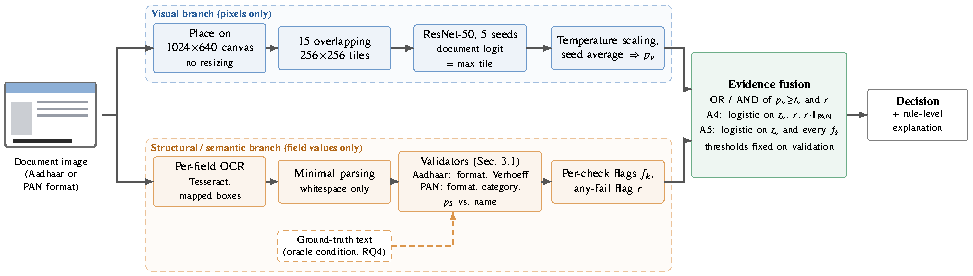
\includegraphics[width=\linewidth,height=0.85\textheight,keepaspectratio]{figure_pdf/Figure1.pdf}\end{center}
\clearpage
\noindent\textbf{FIGURE 2}\par\medskip
\begin{center}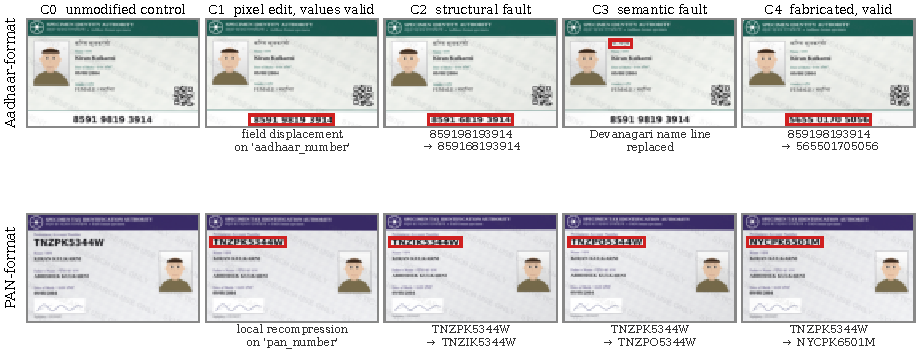
\includegraphics[width=\linewidth,height=0.85\textheight,keepaspectratio]{figure_pdf/Figure2.pdf}\end{center}
\clearpage
\noindent\textbf{FIGURE 3}\par\medskip
\begin{center}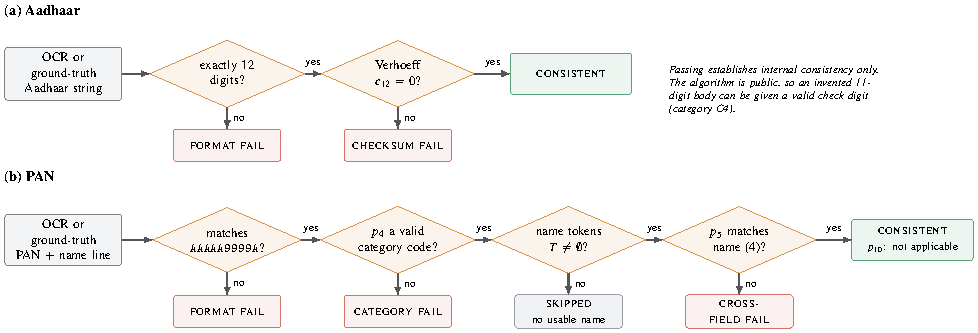
\includegraphics[width=\linewidth,height=0.85\textheight,keepaspectratio]{figure_pdf/Figure3.pdf}\end{center}
\clearpage
\noindent\textbf{FIGURE 4}\par\medskip
\begin{center}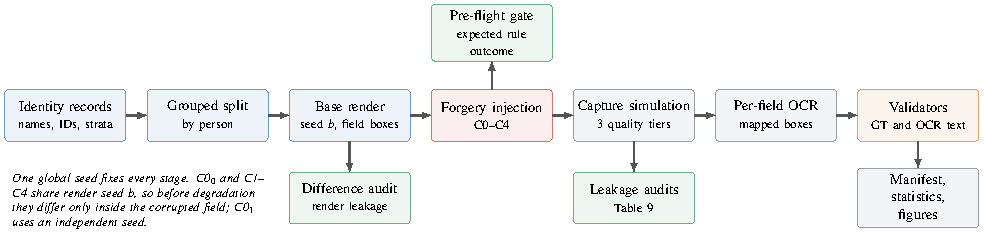
\includegraphics[width=\linewidth,height=0.85\textheight,keepaspectratio]{figure_pdf/Figure4.pdf}\end{center}
\clearpage
\noindent\textbf{FIGURE 5}\par\medskip
\begin{center}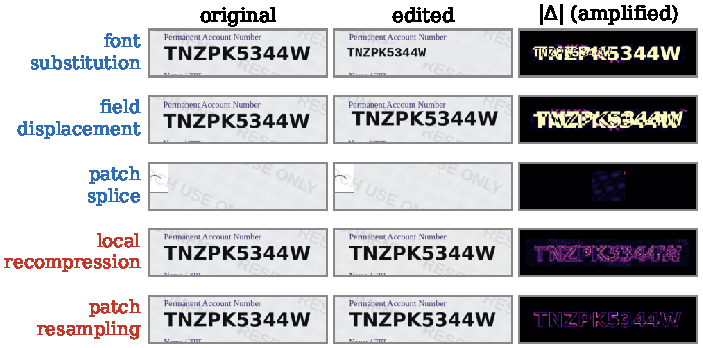
\includegraphics[width=\linewidth,height=0.85\textheight,keepaspectratio]{figure_pdf/Figure5.pdf}\end{center}
\clearpage
\noindent\textbf{FIGURE 6}\par\medskip
\begin{center}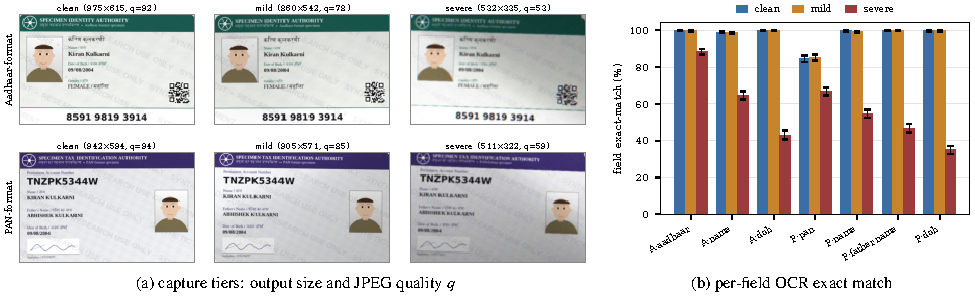
\includegraphics[width=\linewidth,height=0.85\textheight,keepaspectratio]{figure_pdf/Figure6.pdf}\end{center}
\clearpage
\noindent\textbf{FIGURE 7}\par\medskip
\begin{center}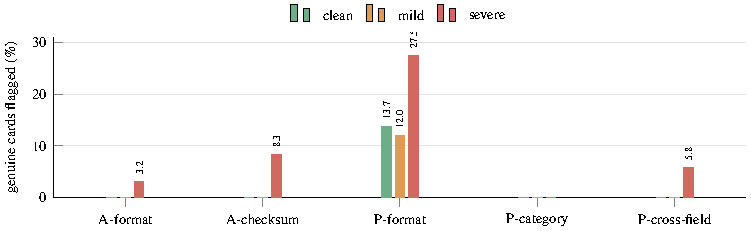
\includegraphics[width=\linewidth,height=0.85\textheight,keepaspectratio]{figure_pdf/Figure7.pdf}\end{center}
\clearpage
\noindent\textbf{FIGURE 8}\par\medskip
\begin{center}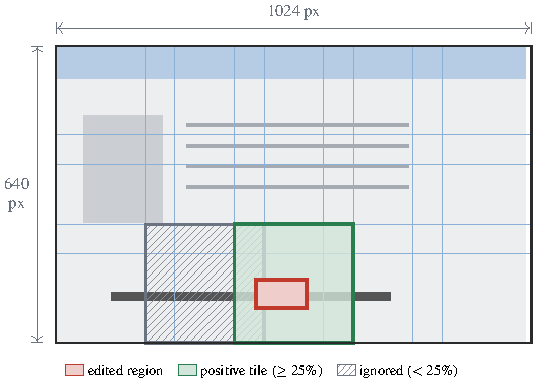
\includegraphics[width=\linewidth,height=0.85\textheight,keepaspectratio]{figure_pdf/Figure8.pdf}\end{center}
\clearpage
\noindent\textbf{FIGURE 9}\par\medskip
\begin{center}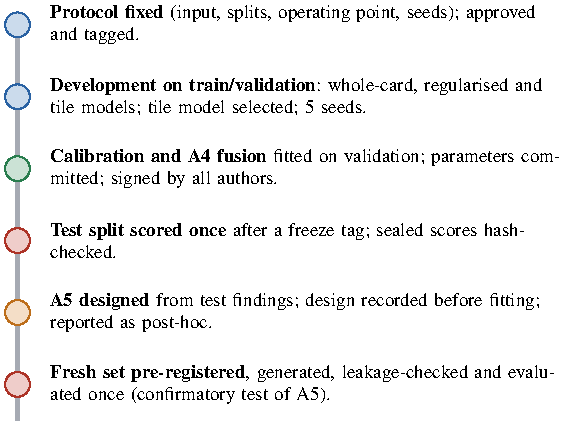
\includegraphics[width=\linewidth,height=0.85\textheight,keepaspectratio]{figure_pdf/Figure9.pdf}\end{center}
\clearpage
\noindent\textbf{FIGURE 10}\par\medskip
\begin{center}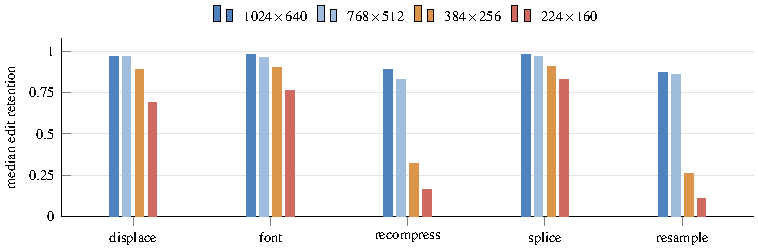
\includegraphics[width=\linewidth,height=0.85\textheight,keepaspectratio]{figure_pdf/Figure10.pdf}\end{center}
\clearpage
\noindent\textbf{FIGURE 11}\par\medskip
\begin{center}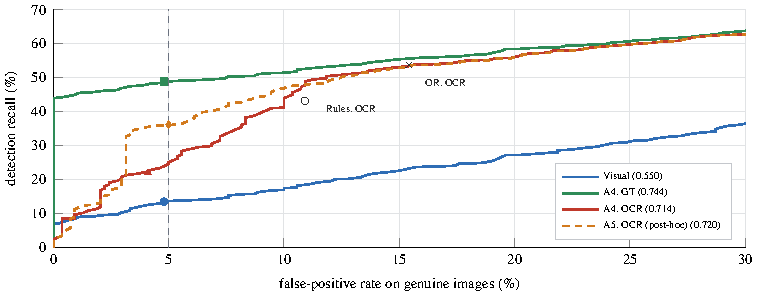
\includegraphics[width=\linewidth,height=0.85\textheight,keepaspectratio]{figure_pdf/Figure11.pdf}\end{center}
\clearpage
\noindent\textbf{FIGURE 12}\par\medskip
\begin{center}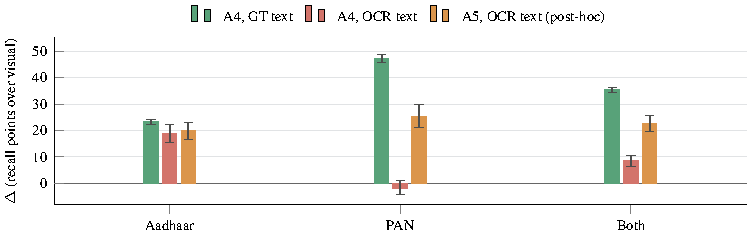
\includegraphics[width=\linewidth,height=0.85\textheight,keepaspectratio]{figure_pdf/Figure12.pdf}\end{center}

\fi
\end{document}
